\chapter{Tinjauan Pustaka}

% ============================================================
\section{Geometri Diferensial}
\label{sec:geometri-diferensial}
% ============================================================

\subsection{Manifold}
\label{subsec:manifold}

Teori relativitas umum mendeskripsikan gravitasi sebagai kelengkungan ruang-waktu. Untuk memformulasikan gagasan ini secara matematis, diperlukan suatu objek yang cukup umum untuk merepresentasikan ruang yang melengkung, tetapi cukup terstruktur untuk memungkinkan operasi kalkulus. Objek tersebut adalah \textit{manifold}: ruang yang secara global bisa melengkung, tetapi secara lokal tampak seperti ruang datar $\mathbb{R}^n$. Sebelum mendefinisikan manifold, terlebih dahulu diperkenalkan konsep ruang topologi yang menjadi fondasinya.

Dalam analisis biasa di $\mathbb{R}^n$, konsep ``dekat'' dan ``jauh'' didefinisikan melalui fungsi jarak. Namun, tidak semua ruang memiliki fungsi jarak yang natural, dan bahkan ketika fungsi jarak ada, banyak sifat penting seperti kontinuitas dan konvergensi sebenarnya hanya bergantung pada struktur yang lebih sederhana, yaitu himpunan-himpunan mana saja yang dianggap ``terbuka.'' Ruang topologi memformalkan gagasan ini dengan menentukan koleksi himpunan terbuka tanpa mengacu pada fungsi jarak eksplisit.

Sebuah ruang topologi adalah pasangan $(X, \tau)$, di mana $X$ adalah suatu himpunan dan $\tau \subseteq \mathcal{P}(X)$ adalah koleksi himpunan bagian dari $X$, disebut himpunan terbuka, yang memenuhi tiga aksioma berikut \cite{nakahara2003geometry}:
\begin{enumerate}[label=\roman*.]
    \item Himpunan kosong dan himpunan total termasuk dalam $\tau$:
    \begin{equation}
        \varnothing \in \tau, \qquad X \in \tau.
    \end{equation}
    \item Gabungan arbitrer dari himpunan-himpunan terbuka adalah himpunan terbuka:
    \begin{equation}
        \{U_\alpha\}_{\alpha \in I} \subseteq \tau
        \quad \Longrightarrow \quad
        \bigcup_{\alpha \in I} U_\alpha \in \tau.
    \end{equation}
    \item Irisan berhingga dari himpunan-himpunan terbuka adalah himpunan terbuka:
    \begin{equation}
        U_1, \ldots, U_n \in \tau
        \quad \Longrightarrow \quad
        \bigcap_{k=1}^{n} U_k \in \tau.
    \end{equation}
\end{enumerate}
Koleksi $\tau$ disebut topologi pada $X$. Jika $x \in U$ dan $U \in \tau$, maka $U$ merupakan lingkungan terbuka dari $x$. Contoh paling mendasar adalah topologi standar pada $\mathbb{R}$, yang dibangun dari gabungan semua interval terbuka $(a, b)$ dengan $a < b$. Konsep ruang topologi diilustrasikan pada Gambar~\ref{fig:ruang-topologi}.

\begin{figure}[H]
\centering
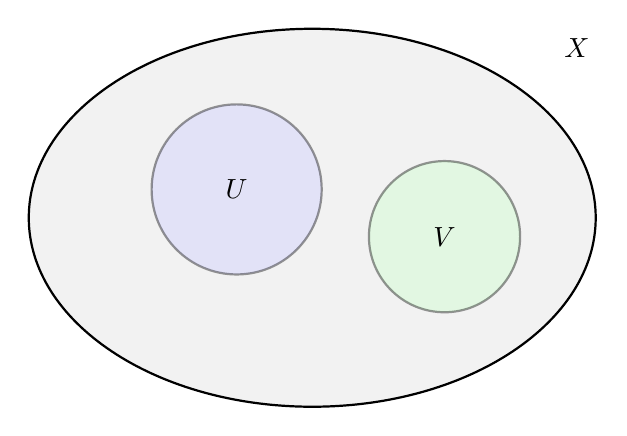
\begin{tikzpicture}[scale=1.2]
  \draw[thick, fill=gray!10] (0,0) ellipse (3cm and 2cm);
  \node at (2.8,1.8) {$X$};
  \draw[thick, fill=blue!20, opacity=0.4] (-0.8,0.3) circle (0.9cm);
  \node at (-0.8,0.3) {$U$};
  \draw[thick, fill=green!20, opacity=0.4] (1.4,-0.2) circle (0.8cm);
  \node at (1.4,-0.2) {$V$};
\end{tikzpicture}
\caption{Ruang topologi $(X, \tau)$ dengan dua himpunan terbuka $U$ dan $V$. Setiap titik di dalam $U$ atau $V$ memiliki lingkungan terbuka yang memuatnya.}
\label{fig:ruang-topologi}
\end{figure}

Dengan ruang topologi sebagai fondasi, manifold didefinisikan sebagai ruang topologi dengan tiga sifat tambahan. Sebuah manifold topologi berdimensi-$n$ adalah ruang topologi $(M, \tau)$ yang memenuhi \cite{nakahara2003geometry, eguchi1980}:
\begin{enumerate}[label=\roman*.]
    \item \textbf{Hausdorff}: untuk setiap $p \neq q$ di $M$, terdapat $U \ni p$ dan $V \ni q$ dengan $U \cap V = \varnothing$.

    \item \textbf{Second countable}: terdapat basis topologi $\mathcal{B} = \{B_i\}_{i \in \mathbb{N}}$ yang dapat dihitung.

    \item \textbf{Lokal-Euclidean berdimensi-$n$}: untuk setiap $p \in M$, terdapat himpunan terbuka $U \subset M$ yang memuat $p$ beserta pemetaan
    \begin{equation}
        \varphi : U \longrightarrow \varphi(U) \subset \mathbb{R}^n,
    \end{equation}
    yang merupakan homeomorfisme (fungsi bijektif kontinu dengan invers kontinu). Pasangan $(U, \varphi)$ disebut \textit{chart}. Koordinat titik $p$ diberikan oleh
    \begin{equation}
        \varphi(p) = (x^1(p),\, x^2(p),\, \ldots,\, x^n(p)) \in \mathbb{R}^n.
    \end{equation}
\end{enumerate}

Masing-masing sifat di atas memiliki peran spesifik. Sifat pertama, Hausdorff, memastikan bahwa setiap dua titik berbeda pada manifold dapat dipisahkan oleh lingkungan terbuka yang saling lepas, sebagaimana diilustrasikan pada Gambar~\ref{fig:hausdorff}. Tanpa sifat ini, suatu barisan bisa konvergen ke lebih dari satu titik sekaligus, sehingga konsep limit dan turunan menjadi ambigu. Dalam konteks gravitasi, ambiguitas semacam ini akan membuat persamaan diferensial pada ruang-waktu tidak konsisten.

\begin{figure}[H]
\centering
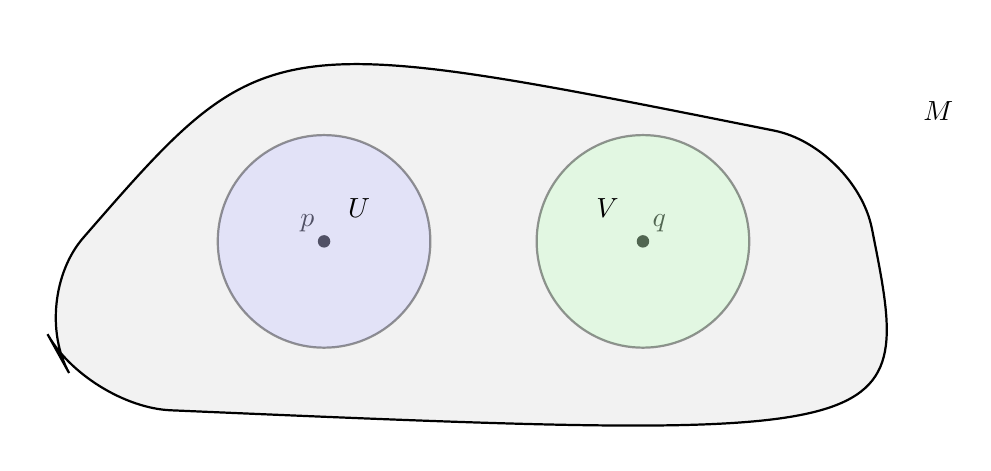
\begin{tikzpicture}[scale=1.5]
  \draw[thick, fill=gray!10, rounded corners=30pt]
    (-4,-0.3) .. controls (-2,2) .. (3,1)
    .. controls (3.5,-1.5) .. (-3.5,-1.2) -- cycle;
  \node at (3.7,1.3) {$M$};
  \fill (-1.5,0.2) circle (1.5pt) node[above left] {$p$};
  \fill ( 1.2,0.2) circle (1.5pt) node[above right] {$q$};
  \draw[thick, fill=blue!20, opacity=0.4] (-1.5,0.2) circle (0.9cm)
    node[above right=5pt, opacity=1] {$U$};
  \draw[thick, fill=green!20, opacity=0.4] ( 1.2,0.2) circle (0.9cm)
    node[above left=5pt, opacity=1] {$V$};
\end{tikzpicture}
\caption{Sifat Hausdorff: titik $p \in U$ dan $q \in V$ dapat dipisahkan oleh lingkungan terbuka yang saling lepas, $U \cap V = \varnothing$.}
\label{fig:hausdorff}
\end{figure}

Sifat kedua, \textit{second countable}, menyatakan bahwa topologi pada manifold dapat dibangun dari basis yang jumlah elemennya terhitung, yaitu koleksi himpunan terbuka $\mathcal{B} = \{B_i\}_{i \in \mathbb{N}}$ sedemikian sehingga setiap himpunan terbuka $U \in \tau$ dapat ditulis sebagai gabungan dari anggota-anggota $\mathcal{B}$, sebagaimana diilustrasikan pada Gambar~\ref{fig:second-countable}. Sifat ini memungkinkan konstruksi partisi kesatuan (\textit{partition of unity}), yaitu alat yang digunakan untuk menjahit objek-objek lokal seperti fungsi atau tensor yang didefinisikan pada masing-masing chart menjadi objek global pada seluruh manifold.

\begin{figure}[H]
\centering
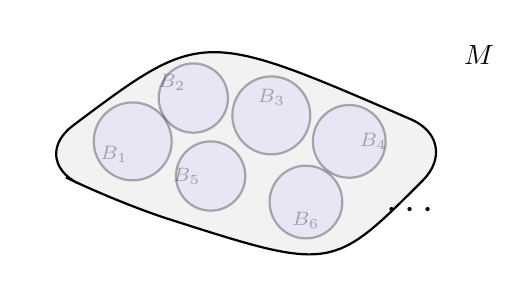
\begin{tikzpicture}[scale=1.1]
  \draw[thick, fill=gray!10, rounded corners=20pt] (-3,0) .. controls (-1,1.5) .. (2,0.2)
     .. controls (0.5,-1.3) .. (-2,-0.5) -- cycle;
  \node at (2.2,1.2) {$M$};
  \draw[thick, fill=blue!20, opacity=0.30] (-1.8,0.2) circle (0.45cm) node[below left=-2pt] {\scriptsize $B_1$};
  \draw[thick, fill=blue!20, opacity=0.30] (-1.1,0.7) circle (0.40cm) node[above left=-1pt] {\scriptsize $B_2$};
  \draw[thick, fill=blue!20, opacity=0.30] (-0.2,0.5) circle (0.45cm) node[above] {\scriptsize $B_3$};
  \draw[thick, fill=blue!20, opacity=0.30] ( 0.7,0.2) circle (0.42cm) node[right] {\scriptsize $B_4$};
  \draw[thick, fill=blue!20, opacity=0.30] (-0.9,-0.2) circle (0.40cm) node[left] {\scriptsize $B_5$};
  \draw[thick, fill=blue!20, opacity=0.30] ( 0.2,-0.5) circle (0.42cm) node[below] {\scriptsize $B_6$};
  \node at (1.4,-0.6) {\Large $\cdots$};
\end{tikzpicture}
\caption{Sifat \textit{second countable}: terdapat basis topologi $\{B_i\}_{i \in \mathbb{N}}$ yang terhitung. Setiap himpunan terbuka pada manifold dapat dinyatakan sebagai gabungan dari elemen-elemen basis ini.}
\label{fig:second-countable}
\end{figure}

Sifat ketiga, lokal-Euclidean, merupakan inti dari definisi manifold. Sifat ini menyatakan bahwa meskipun manifold $M$ dapat memiliki struktur global yang kompleks, di sekitar setiap titik $p$ terdapat lingkungan terbuka $U$ yang dapat dipetakan secara homeomorfik ke himpunan terbuka di $\mathbb{R}^n$. Pemetaan $\varphi : U \to \varphi(U) \subset \mathbb{R}^n$ memberikan label koordinat $(x^1, \ldots, x^n)$ untuk setiap titik dalam $U$, sehingga semua operasi kalkulus dapat dilakukan di $\mathbb{R}^n$ melalui chart ini, meskipun manifold itu sendiri bukan ruang Euclidean secara global. Untuk gravitasi $2+1$ dimensi, manifold ruang-waktu yang digunakan berdimensi $n = 3$.

Satu chart umumnya tidak cukup untuk menutupi seluruh manifold. Sebagai contoh, permukaan bola $S^2$ tidak dapat ditutupi oleh satu chart tunggal. Kumpulan chart yang menutupi seluruh manifold disebut atlas:
\begin{equation}
    \mathcal{A} = \{(U_\alpha,\, \varphi_\alpha)\}_{\alpha \in I}, \qquad \bigcup_{\alpha \in I} U_\alpha = M.
\end{equation}
Jika dua chart $(U, \varphi)$ dan $(V, \psi)$ saling beririsan ($U \cap V \neq \varnothing$), satu titik $p \in U \cap V$ memiliki dua representasi koordinat: $x = \varphi(p)$ dan $y = \psi(p)$. Konsistensi antar kedua sistem koordinat dijamin oleh peta transisi:
\begin{equation}\label{eq:transition-map}
    \omega = \psi \circ \varphi^{-1} : \varphi(U \cap V) \longrightarrow \psi(U \cap V),
\end{equation}
beserta inversnya $\omega^{-1} = \varphi \circ \psi^{-1}$. Secara skematis, proses perpindahan koordinat berlangsung sebagai
\begin{equation}
    U\cap V 
    \;\xrightarrow{\;\varphi\;}\; 
    \varphi(U\cap V)
    \;\xrightarrow[\text{peta transisi}]{\;\omega = \psi\circ\varphi^{-1}\;}
    \psi(U\cap V)
    \;\xleftarrow{\;\psi\;}\;
    U\cap V.
\end{equation}
Titik $p \in U \cap V$ pertama-tama dipetakan oleh $\varphi$ menjadi koordinat $x = \varphi(p)$ di $\mathbb{R}^n$, kemudian koordinat ini dikonversi ke sistem koordinat chart $\psi$ melalui $\omega(x) = \psi(\varphi^{-1}(x))$, sehingga diperoleh $y = \psi(p)$. Manifold disebut halus (\textit{smooth}) jika setiap peta transisi dan inversnya berkelas $C^\infty$ \cite{nakahara2003geometry}. Kondisi ini memastikan bahwa perpindahan antar koordinat berlangsung halus tanpa diskontinuitas, sehingga kalkulus diferensial dapat dilakukan secara konsisten di seluruh manifold. Gambar~\ref{fig:lokal-euclidean} mengilustrasikan seluruh konstruksi ini pada contoh manifold $S^2$.

\begin{figure}[H]
\centering
\begin{tikzpicture}[scale=0.95,>=Latex]
  \colorlet{Ucol}{blue!55}
  \colorlet{Vcol}{green!55}
  \colorlet{Wcol}{brown!65}
  \tikzset{
    lab/.style={scale=0.92},
    smalllab/.style={scale=0.85},
    axis/.style={->,thin},
    regU/.style={fill=Ucol, draw=Ucol!50!black, opacity=0.55},
    regV/.style={fill=Vcol, draw=Vcol!50!black, opacity=0.55},
    regWfill/.style={fill=Wcol, opacity=0.55},
    regWdraw/.style={draw=Wcol!80!black, dashed, line width=0.8pt},
  }
  \def\PatchPhiU{
    plot[smooth,tension=0.7] coordinates {
      (1.9,1.3) (2.6,1.2) (3.6,1.4) (4.1,1.8) (4.2,2.5)
      (3.7,2.8) (2.8,2.9) (2.1,2.6) (1.8,1.9) (1.9,1.3)
    } -- cycle
  }
  \def\PatchVtoPhi{
    plot[smooth,tension=0.8] coordinates {
      (1.7,1.35) (2.35,1.15) (2.95,1.35) (3.15,1.75)
      (3.05,2.15) (2.55,2.30) (2.05,2.25) (1.75,1.85) (1.7,1.35)
    } -- cycle
  }
  \def\PatchPsiV{
    plot[smooth,tension=0.7] coordinates {
      (0.9,0.8) (1.7,0.7) (2.8,0.9) (3.3,1.3) (3.4,2.0)
      (2.9,2.4) (2.0,2.5) (1.2,2.1) (0.8,1.4) (0.9,0.8)
    } -- cycle
  }
  \def\PatchUtoPsi{
    plot[smooth,tension=0.8] coordinates {
      (2.35,1.65) (2.85,1.55) (3.25,1.75) (3.30,2.10)
      (3.00,2.35) (2.55,2.40) (2.35,2.10) (2.30,1.80) (2.35,1.65)
    } -- cycle
  }
  \coordinate (C) at (0,5);
  \shade[ball color=gray!20,opacity=0.3] (C) circle (1.8cm);
  \draw[thick] (C) circle (1.8cm);
  \draw[thick] (C) ellipse (1.8cm and 0.6cm);
  \draw[thick,dashed] (C) ellipse (0.6cm and 1.8cm);
  \node[lab] at (2.5,6.5) {$M=S^2$};
  \begin{scope}
    \clip (C) circle (1.8cm);
    \fill[regV] (-0.6,4.4) ellipse (1.0cm and 0.85cm);
    \draw[regV] (-0.6,4.4) ellipse (1.0cm and 0.85cm);
  \end{scope}
  \begin{scope}
    \clip (C) circle (1.8cm);
    \fill[regU] (0.5,5.5) ellipse (0.95cm and 0.8cm);
    \draw[regU] (0.5,5.5) ellipse (0.95cm and 0.8cm);
  \end{scope}
  \begin{scope}
    \clip (C) circle (1.8cm);
    \clip (0.5,5.5) ellipse (0.95cm and 0.8cm);
    \clip (-0.6,4.4) ellipse (1.0cm and 0.85cm);
    \fill[regWfill] (-2,3) rectangle (3,7);
  \end{scope}
  \begin{scope}
    \clip (C) circle (1.8cm);
    \clip (0.5,5.5) ellipse (0.95cm and 0.8cm);
    \draw[regWdraw] (-0.6,4.4) ellipse (1.0cm and 0.85cm);
  \end{scope}
  \begin{scope}
    \clip (C) circle (1.8cm);
    \clip (-0.6,4.4) ellipse (1.0cm and 0.85cm);
    \draw[regWdraw] (0.5,5.5) ellipse (0.95cm and 0.8cm);
  \end{scope}
  \node[lab, text=Ucol!60!black] at (1.0,5.8) {$U$};
  \node[lab, text=Vcol!60!black] at (-1.1,4.2) {$V$};
  \node[smalllab, text=Wcol!80!black] at (-0.05,5.0) {$U\cap V$};
  \draw[->,thick,Ucol!80!black] (0.8,5.3)
    .. controls (-1.0,3.5) and (-2.5,2.5) .. (-4.5,1.0)
    node[pos=0.45,left,lab] {$\varphi$};
  \draw[->,thick,Vcol!80!black] (-0.8,4.5)
    .. controls (1.5,3.0) and (3.0,2.0) .. (4.5,1.0)
    node[pos=0.45,right,lab] {$\psi$};
  \begin{scope}[shift={(-7.5,-0.5)}]
    \node[lab,anchor=south] at (2.5,3.5) {$\mathbb{R}^2$};
    \draw[axis] (-0.3,0) -- (5.5,0) node[below right] {$x^1$};
    \draw[axis] (0,-0.3) -- (0,3.5) node[above left] {$x^2$};
    \draw[gray!30,very thin] (0,0) grid (5,3);
    \draw[thick,Ucol!80!black,fill=Ucol!15] \PatchPhiU;
    \node[lab, text=Ucol!80!black] at (3.3,2.3) {$\varphi(U)$};
    \draw[opacity=0] \PatchVtoPhi;
    \begin{scope} \clip \PatchPhiU; \clip \PatchVtoPhi;
      \fill[regWfill] (0,0) rectangle (5.5,3.5); \end{scope}
    \begin{scope} \clip \PatchPhiU; \draw[regWdraw] \PatchVtoPhi; \end{scope}
    \begin{scope} \clip \PatchVtoPhi; \draw[regWdraw] \PatchPhiU; \end{scope}
    \node[smalllab, text=Wcol!80!black] at (2.35,1.75) {$\varphi(U\cap V)$};
  \end{scope}
  \begin{scope}[shift={(2.0,-0.5)}]
    \node[lab,anchor=south] at (2.5,3.5) {$\mathbb{R}^2$};
    \draw[axis] (-0.3,0) -- (5.5,0) node[below right] {$y^1$};
    \draw[axis] (0,-0.3) -- (0,3.5) node[above left] {$y^2$};
    \draw[gray!30,very thin] (0,0) grid (5,3);
    \draw[thick,Vcol!80!black,fill=Vcol!15] \PatchPsiV;
    \node[lab, text=Vcol!80!black] at (1.7,1.5) {$\psi(V)$};
    \draw[opacity=0] \PatchUtoPsi;
    \begin{scope} \clip \PatchPsiV; \clip \PatchUtoPsi;
      \fill[regWfill] (0,0) rectangle (5.5,3.5); \end{scope}
    \begin{scope} \clip \PatchPsiV; \draw[regWdraw] \PatchUtoPsi; \end{scope}
    \begin{scope} \clip \PatchUtoPsi; \draw[regWdraw] \PatchPsiV; \end{scope}
    \node[smalllab, text=Wcol!80!black] at (2.75,2.0) {$\psi(U\cap V)$};
  \end{scope}
  \draw[->,very thick,Wcol!80!black] (-2.7,1.0)
    .. controls (-1.4,0.5) and (-0.7,0.5) .. (0.3,1.0);
  \node[smalllab, text=Wcol!90!black,align=center] at (-1.2,0.1)
    {$\omega=\psi\circ\varphi^{-1}$\\[-2pt]\scriptsize(peta transisi)};
  \draw[->,very thick,Wcol!80!black] (0.3,0.1)
    .. controls (-0.7,-0.4) and (-1.4,-0.4) .. (-2.7,0.1);
  \node[smalllab, text=Wcol!90!black] at (-0.3,-0.5)
    {$\omega^{-1}=\varphi\circ\psi^{-1}$};
\end{tikzpicture}
\caption{Sifat lokal-Euclidean dan peta transisi pada manifold $S^2$. Dua chart $(U, \varphi)$ dan $(V, \psi)$ masing-masing memetakan bagian manifold ke $\mathbb{R}^2$. Pada daerah irisan $U \cap V$ (coklat), peta transisi $\omega = \psi \circ \varphi^{-1}$ menghubungkan kedua sistem koordinat secara halus.}
\label{fig:lokal-euclidean}
\end{figure}

\subsection{Ruang Singgung, Kotangen, dan Tensor Metrik}
\label{subsec:tangent-cotangent}

Setelah manifold terdefinisi, perlu dibangun cara untuk mendeskripsikan arah dan kecepatan pada ruang yang melengkung. Dalam ruang datar $\mathbb{R}^n$, vektor dapat didefinisikan sebagai ``panah'' yang menghubungkan dua titik. Pada manifold yang melengkung, cara ini tidak lagi berlaku karena tidak ada cara natural untuk membandingkan posisi dua titik yang terpisah. Solusinya adalah mendefinisikan vektor secara lokal, yaitu sebagai arah gerak dari suatu lintasan halus yang melewati titik tersebut. Dengan pendekatan ini, definisi vektor tidak bergantung pada cara manifold dibenamkan (\textit{embedded}) dalam ruang luar.


\vspace{0.5em}
\noindent \textbf{Lintasan halus pada manifold}

Misalkan terdapat sebuah interval terbuka $(-\varepsilon, \varepsilon) \subset \mathbb{R}$ dan peta halus (\textit{smooth map})
\begin{equation}
    c : (-\varepsilon, \varepsilon) \longrightarrow M, \qquad c(0) = p.
\end{equation}
Setiap $t \in (-\varepsilon, \varepsilon)$ dipetakan ke satu titik $c(t) \in M$. Titik $p = c(0)$ adalah posisi di manifold tempat lintasan melewati pada $t = 0$. Himpunan nilai balik (\textit{preimage}) dari titik-titik di sekitar $t = 0$ membentuk lintasan halus $c(t)$ di dalam manifold $M$. Secara intuitif, lintasan $c(t)$ dapat dipandang sebagai gerak partikel yang bergerak di atas permukaan manifold seiring perubahan parameter $t$.

Untuk mengekstrak ``arah gerak'' partikel di titik $p$, digunakan koordinat lokal $\varphi : U \to \mathbb{R}^n$ dengan $x^i = \varphi^i(p)$. Komposisi $\varphi \circ c : (-\varepsilon, \varepsilon) \to \mathbb{R}^n$ adalah fungsi biasa dari $\mathbb{R}$ ke $\mathbb{R}^n$ yang dapat diturunkan secara standar. Seluruh konstruksi ini diilustrasikan pada Gambar~\ref{fig:lintasan}: parameter $t$ di interval dipetakan oleh $c$ ke manifold $M$, kemudian chart $\varphi$ membawanya ke $\mathbb{R}^n$, dan komposisi $\varphi \circ c$ adalah fungsi yang ``siap diturunkan.''

\begin{figure}[H]
\centering
\begin{tikzpicture}[scale=1.05,>=Latex]
  \tikzset{lab/.style={scale=0.9}, smalllab/.style={scale=0.8}}
  \draw[thick,rounded corners=20pt]
    (-2,0) .. controls (-1,2.5) and (2,2.2) .. (3,1.2)
    .. controls (2,-0.8) and (-1,-1.2) .. (-2,0);
  \node[lab] at (3.3,1.6) {$M$};
  \draw[thick,blue!40,fill=blue!15,opacity=0.6,rounded corners=10pt]
    (0.3,0.3) ellipse (1.2cm and 0.7cm);
  \node[lab,blue!70!black] at (1.6,1.1) {$U$};
  \draw[red!70,thick]
    (-0.8,0.55) .. controls (0.3,1.0) and (0.6,0.15) .. (1.2,0.9);
  \node[lab,red!70!black] at (1.05,1.25) {$c(t)$};
  \coordinate (ct) at (0.3,0.60);
  \fill (ct) circle (2pt);
  \node[above right=-2pt,scale=0.9] at (ct) {$c(0)=p$};
  \coordinate (a) at (-3,0.8); \coordinate (b) at (-3,2.2);
  \draw[thick] (a) -- (b);
  \node[left] at (a) {$-\varepsilon$}; \node[left] at (b) {$\varepsilon$};
  \node[left,scale=0.9] at (-3,1.5) {$t$};
  \draw[->,thick] (-2.9,1.5) .. controls (-1.3,1.1) and (-0.4,0.9) .. (0.4,0.8);
  \node[above,scale=0.9] at (-1.2,1.25) {$c$};
  \draw[->,thick] (0.7,0.8) .. controls (1.5,0.2) and (2.0,-0.4) .. (2.3,-1.0);
  \node[right,scale=0.9] at (1.5,-0.1) {$\varphi$};
  \draw[->,thick] (2.4,-3.3) -- (4.6,-3.3) node[right,smalllab] {$x^1$};
  \draw[->,thick] (2.4,-3.3) -- (2.4,-1.5) node[above,smalllab] {$x^2$};
  \draw[red!70,thick,smooth]
    (2.4,-3.0) .. controls (3.1,-2.7) and (3.6,-2.9) .. (4.3,-2.5);
  \fill (3.3,-2.75) circle (1.5pt);
  \node[above right=-2pt,scale=0.9] at (3.3,-2.75) {$\varphi(c(0))$};
  \node[lab,red!70!black] at (4.9,-3) {$\varphi\circ c(t)$};
  \draw[->,thick,dashed] (-2.9,1.5) .. controls (-1.0,-0.3) and (1.0,-1.5) .. (2.3,-2.3);
  \node[lab] at (0.7,-1) {$\varphi\circ c$};
\end{tikzpicture}
\caption{Lintasan $c(t)$ memetakan interval $(-\varepsilon, \varepsilon)$ ke manifold $M$. Chart $\varphi$ kemudian membawa lintasan ini ke $\mathbb{R}^n$, menghasilkan fungsi $\varphi \circ c(t)$ yang dapat diturunkan secara biasa.}
\label{fig:lintasan}
\end{figure}


\vspace{0.5em}
\noindent \textbf{Vektor singgung dari lintasan}

Dari lintasan halus $c(t)$ dengan $c(0) = p$, vektor singgung di titik $p$ didefinisikan melalui aksinya pada fungsi halus $f : M \to \mathbb{R}$. Perubahan nilai $f$ sepanjang lintasan $c(t)$ diberikan oleh:
\begin{equation}\label{eq:tangent-action-f}
    v(f) = \frac{d}{dt}\bigg|_{t=0} f(c(t)),
    \qquad v \in T_pM.
\end{equation}
Mengapa bentuknya seperti ini? Pada manifold, fungsi $f$ tidak bisa langsung diturunkan terhadap ``posisi'' karena manifold bukan $\mathbb{R}^n$. Namun, $f(c(t))$ adalah fungsi komposisi dari $\mathbb{R}$ ke $\mathbb{R}$ (melalui lintasan $c$), yang bisa diturunkan terhadap parameter $t$ secara standar. Besaran $v(f)$ menyatakan laju perubahan $f$ ketika bergerak melalui $p$ mengikuti arah lintasan $c(t)$, dan hasilnya tidak bergantung pada pilihan koordinat: vektor $v$ didefinisikan melalui bagaimana ia mengubah nilai fungsi, bukan melalui komponen-komponennya dalam suatu chart tertentu.

\vspace{0.5em}
\noindent \textbf{Representasi komponen dalam koordinat lokal}

Untuk memperoleh komponen eksplisit dari vektor singgung, digunakan koordinat lokal $\varphi : U \to \mathbb{R}^n$ dengan $x^i = \varphi^i(p)$. Komposisi $f \circ \varphi^{-1}$ adalah fungsi dari $\mathbb{R}^n$ ke $\mathbb{R}$ yang dapat diturunkan secara biasa, sehingga aturan rantai (\textit{chain rule}) dapat diterapkan:
\begin{equation}\label{eq:chain-rule}
    v(f)
    = \frac{d}{dt}\bigg|_{t=0} f(c(t))
    = \frac{d}{dt}\bigg|_{t=0} \big(f \circ \varphi^{-1}\big)\big(\varphi(c(t))\big)
    = \sum_{i=1}^{n}
      \underbrace{\frac{\partial(f \circ \varphi^{-1})}{\partial x^i}\bigg|_{\varphi(p)}}_{\displaystyle \frac{\partial f}{\partial x^i}\big|_p}
      \underbrace{\frac{dx^i}{dt}\bigg|_{t=0}}_{\displaystyle v^i}.
\end{equation}
Langkah kedua menggunakan fakta bahwa $f(c(t)) = (f \circ \varphi^{-1})(\varphi(c(t)))$ karena $c(t) = \varphi^{-1}(\varphi(c(t)))$. Langkah ketiga adalah aturan rantai multivariabel, di mana turunan terhadap $t$ dipecah menjadi turunan terhadap masing-masing koordinat $x^i$ dikalikan laju perubahan koordinat $dx^i/dt$.

Dari persamaan~\eqref{eq:chain-rule}, vektor singgung di titik $p$ ditulis sebagai kombinasi linear dari operator turunan parsial yang bertindak sebagai basis, dikalikan dengan komponen vektor:
\begin{equation}\label{eq:tangent-vector}
    v = \frac{\partial}{\partial x^i}\bigg|_p v^i, \qquad
    v^i \equiv \frac{dx^i}{dt}\bigg|_{t=0}.
\end{equation}
Dalam konvensi sumasi Einstein, persamaan ini dapat juga ditulis sebagai $v = \partial_i\, v^i$. Komponen $v^i$ menyatakan laju perubahan koordinat ke-$i$ sepanjang lintasan pada $t = 0$. Himpunan operator $\{\partial/\partial x^i|_p\}$ membentuk basis untuk ruang singgung $T_pM$, yang merupakan ruang vektor berdimensi-$n$:
\begin{equation}
    T_pM = \mathrm{span}\left\{\frac{\partial}{\partial x^1}\bigg|_p, \ldots, \frac{\partial}{\partial x^n}\bigg|_p\right\} \cong \mathbb{R}^n.
\end{equation}
Secara geometris, $T_pM$ adalah ruang vektor ``datar'' yang menempel pada manifold di titik $p$, sebagaimana ditunjukkan pada Gambar~\ref{fig:tangent-vector}.

\begin{figure}[H]
\centering
\begin{tikzpicture}[scale=1.05,>=Latex]
  \tikzset{
    lab/.style={scale=0.9, inner sep=1.2pt, text=black!90},
    vctr/.style={->,thick,red!70},
    manifold/.style={thick,rounded corners=18pt,fill=gray!10}
  }
  \draw[manifold]
    (-2,0) .. controls (-1,2.0) and (1.5,1.6) .. (2.6,0.8)
    .. controls (1.5,-0.8) and (-1,-1.0) .. (-2,0);
  \node[lab] at (2.8,1.45) {$M$};
  \draw[thick,red!70,smooth]
    (-1.3,0.25) .. controls (-0.6,0.8) and (0.8,0.95) .. (1.5,0.25);
  \node[lab,red!70!black,anchor=south west] at (1.1,0.95) {$c(t)$};
  \coordinate (p) at (0.35,0.68);
  \fill (p) circle (1.5pt);
  \node[lab,anchor=south east] at ([xshift=-2pt,yshift=4pt]p) {$p=c(0)$};
  \draw[dashed,thick] (-1.6,0.68) -- (1.9,0.68);
  \node[lab,anchor=north] at (0.3,0.48) {$T_pM$};
  \draw[vctr] (p) -- ++(0.9,0.2)
    node[lab,anchor=west,xshift=2pt,yshift=2pt] {$v=\tfrac{dc}{dt}\big|_{0}$};
\end{tikzpicture}
\caption{Vektor singgung $v = dc/dt|_{t=0}$ di titik $p$ merupakan elemen ruang singgung $T_pM$. Ruang $T_pM$ secara geometris adalah bidang datar yang menyinggung manifold di titik $p$.}
\label{fig:tangent-vector}
\end{figure}

\vspace{0.5em}
\noindent \textbf{Vektor sebagai operator diferensial}

Persamaan~\eqref{eq:tangent-vector} menunjukkan bahwa vektor singgung bukan sekadar $n$-tupel bilangan $(v^1, \ldots, v^n)$, melainkan operator diferensial yang beraksi pada fungsi halus. Jika $X$ adalah vektor singgung di titik $p$ yang berkorespondensi dengan lintasan $c(t)$, maka:
\begin{equation}\label{eq:operator-X}
    X = \frac{\partial}{\partial x^i}\bigg|_p X^i, \qquad X^i = \frac{dx^i}{dt}\bigg|_{t=0},
\end{equation}
dan aksi $X$ pada fungsi $f : M \to \mathbb{R}$ diberikan oleh
\begin{equation}\label{eq:vec-action}
    X[f] = \frac{\partial f}{\partial x^i}\bigg|_p X^i.
\end{equation}
Besaran $X[f]$ adalah turunan arah (\textit{directional derivative}), yaitu laju perubahan $f$ sepanjang arah $X$. Meskipun komponen $X^i$ bergantung pada pilihan chart, hasil aksi $X[f]$ selalu sama untuk semua chart, sehingga definisi ini bersifat koordinat-independen.

\vspace{0.5em}
\vspace{0.5em}
\noindent \textbf{Ruang kotangen}

Setelah ruang singgung terdefinisi, langkah berikutnya adalah membangun ruang dualnya. Jika vektor singgung merepresentasikan ``arah gerak,'' maka objek dual yang mengukur besaran fisis sepanjang arah tersebut adalah kovektor atau 1-form.

Secara umum, untuk setiap ruang vektor $V$, dapat didefinisikan ruang dual $V^*$ yang terdiri dari seluruh pemetaan linear dari $V$ ke $\mathbb{R}$. Himpunan pemetaan linear semacam ini dinotasikan $\mathrm{Hom}(V, \mathbb{R})$, di mana ``Hom'' adalah singkatan dari \textit{homomorphism}, yaitu peta yang menjaga struktur linear (penjumlahan dan perkalian skalar). Dengan kata lain, $\omega \in V^*$ adalah fungsi $\omega : V \to \mathbb{R}$ yang memenuhi $\omega(\alpha u + \beta v) = \alpha\,\omega(u) + \beta\,\omega(v)$ untuk semua $u, v \in V$ dan $\alpha, \beta \in \mathbb{R}$.

Menerapkan konstruksi ini pada ruang singgung, ruang kotangen $T_p^*M$ didefinisikan sebagai \cite{nakahara2003geometry}:
\begin{equation}
    T_p^*M = \mathrm{Hom}(T_pM, \mathbb{R}) = \{\omega : T_pM \to \mathbb{R} \mid \omega\ \text{linear}\}.
\end{equation}
Elemen $\omega \in T_p^*M$ disebut kovektor atau 1-form. Basis ruang kotangen $\{dx^i\}$ memenuhi relasi dualitas
\begin{equation}\label{eq:duality}
    dx^i\!\left(\frac{\partial}{\partial x^j}\right) = \delta^i_{\ j},
\end{equation}
yang menyatakan bahwa basis kovektor $dx^i$ ``menyaring'' komponen ke-$i$ dari vektor: ketika $dx^i$ beraksi pada basis $\partial/\partial x^j$, hasilnya bernilai 1 jika $i = j$ dan 0 jika tidak. Setiap kovektor diekspansi sebagai $\omega = \omega_i \, dx^i$, dan aksinya pada vektor $v = \partial_j\, v^j$ adalah $\omega(v) = \omega_i v^i$. Contoh fundamental dari kovektor adalah diferensial fungsi:
\begin{equation}
    df = \frac{\partial f}{\partial x^i} dx^i, \qquad df(v) = v[f].
\end{equation}
Persamaan terakhir menunjukkan konsistensi antara pandangan vektor sebagai operator turunan arah~\eqref{eq:vec-action} dan diferensial sebagai kovektor: aksi kovektor $df$ pada vektor $v$ menghasilkan bilangan yang sama dengan aksi operator $v$ pada fungsi $f$.

Di bawah transformasi koordinat $x^i \to x'^i(x)$ dengan matriks Jacobian $J^i_{\ j} = \partial x'^i/\partial x^j$, komponen vektor dan kovektor bertransformasi sebagai \cite{carroll2019spacetime}
\begin{equation}\label{eq:contravariant}
    v'^i = \frac{\partial x'^i}{\partial x^j}\, v^j, \qquad
    \omega'_i = \omega_j \frac{\partial x^j}{\partial x'^i}.
\end{equation}
Vektor disebut kontravarian (komponen bertransformasi dengan $J$), kovektor disebut kovarian (bertransformasi dengan $J^{-1}$). \textit{Inner product} antara keduanya invarian terhadap perubahan koordinat:
\begin{equation}
    \omega'_i v'^i = \omega_j v^k \underbrace{\frac{\partial x^j}{\partial x'^i} \frac{\partial x'^i}{\partial x^k}}_{\delta^j_{\ k}} = \omega_j v^j.
\end{equation}

\vspace{0.5em}
\noindent \textbf{Tensor metrik}

Ruang singgung dan ruang kotangen yang telah didefinisikan di atas memberikan bahasa untuk menyatakan arah (vektor) dan besaran yang diukur sepanjang arah tertentu (kovektor). Namun, sejauh ini belum ada cara untuk mengukur \textit{jarak} antar titik atau \textit{sudut} antara dua vektor, karena manifold diferensiabel secara umum tidak memiliki konsep panjang bawaan. Untuk itu diperlukan struktur tambahan berupa tensor metrik, yang mengubah manifold diferensiabel menjadi manifold (pseudo-)Riemannian. Tensor metrik adalah tensor kovarian simetris tipe $(0,2)$:
\begin{equation}\label{eq:metric}
    g = g_{\mu\nu}\, dx^\mu \otimes dx^\nu, \qquad g_{\mu\nu} = g_{\nu\mu}, \quad \det(g_{\mu\nu}) \neq 0.
\end{equation}
Tensor metrik mendefinisikan \textit{inner product} antara dua vektor, $g(v, w) = g_{\mu\nu} v^\mu w^\nu$, yang memungkinkan pengukuran panjang ($|v| = \sqrt{|g(v,v)|}$) dan sudut antar vektor. Selain itu, metrik juga memungkinkan identifikasi antara vektor dan kovektor melalui operasi menaikkan dan menurunkan indeks: $v_\mu = g_{\mu\nu}v^\nu$ dan $\omega^\mu = g^{\mu\nu}\omega_\nu$, dengan $g^{\mu\nu}$ adalah invers dari $g_{\mu\nu}$.

Elemen garis (\textit{line element}) yang menyatakan jarak infinitesimal antara dua titik berdekatan diberikan oleh:
\begin{equation}
    ds^2 = g_{\mu\nu}\, dx^\mu dx^\nu.
\end{equation}
Sebagai contoh, untuk ruang-waktu Minkowski $2+1$ dimensi dengan signatur $(+,-,-)$, elemen garis adalah $ds^2 = dt^2 - dx^2 - dy^2$ dengan metrik $g_{\mu\nu} = \eta_{\mu\nu} = \mathrm{diag}(+1,-1,-1)$. Signatur ini membedakan arah waktu (positif) dari arah ruang (negatif), yang merupakan ciri khas ruang-waktu Lorentzian. Mulai dari sini, indeks Yunani ($\mu, \nu = 0, 1, 2$) digunakan untuk koordinat ruang-waktu dan indeks Latin ($a, b = 0, 1, 2$) untuk kerangka Lorentz lokal.

\section{Kalkulus Eksterior}
\label{sec:kalkulus-eksterior}
% ============================================================

Kovektor atau 1-form mengukur besaran fisis sepanjang satu arah vektor. Namun, dalam fisika sering kali diperlukan objek yang mengukur besaran pada bidang atau volume, bukan hanya sepanjang satu arah. Sebagai contoh, fluks medan listrik melalui suatu permukaan memerlukan objek yang ``memakan'' dua vektor (menentukan bidang) dan menghasilkan bilangan. Kalkulus eksterior menyediakan kerangka untuk mengkonstruksi objek-objek semacam ini secara sistematis melalui bentuk diferensial (\textit{differential forms}), beserta aturan perkalian (\textit{wedge product}) dan turunan (\textit{exterior derivative}) yang sesuai.

\subsection{Bentuk Diferensial dan Wedge Product}
\label{subsec:forms-wedge}

Titik awal kalkulus eksterior adalah menggeneralisasi konsep kovektor. Sebuah 1-form $\omega \in T_p^*M$ menerima satu vektor dan menghasilkan bilangan real. Untuk membangun objek yang menerima dua vektor, tiga vektor, atau $p$ vektor sekaligus, diperkenalkan $p$-form, yaitu pemetaan multilinear dan antisimetrik pada titik $x \in M$ \cite{eguchi1980}:
\begin{equation}
    \omega_x : \underbrace{T_xM \times \cdots \times T_xM}_{p} \longrightarrow \mathbb{R}.
\end{equation}
Sifat multilinear berarti $\omega$ linear terhadap masing-masing argumen vektor. Sifat antisimetrik berarti menukar urutan dua argumen vektor mengubah tanda hasilnya: $\omega(\ldots, u, \ldots, v, \ldots) = -\omega(\ldots, v, \ldots, u, \ldots)$. Sifat antisimetri ini mengkodekan konsep orientasi, karena tanda berubah ketika orientasi bidang atau volume dibalik.

Himpunan semua $p$-form di titik $x$ membentuk ruang vektor $\Lambda^p T_x^*M$ berdimensi $\binom{n}{p}$. Dalam koordinat lokal, $p$-form diekspansi sebagai:
\begin{equation}\label{eq:p-form-coords}
    \omega = \frac{1}{p!}\, \omega_{i_1 \cdots i_p}(x)\, dx^{i_1} \wedge \cdots \wedge dx^{i_p},
\end{equation}
dengan koefisien $\omega_{i_1 \cdots i_p}$ antisimetrik total. Faktor $1/p!$ mengkompensasi penjumlahan berlebih (\textit{overcounting}) akibat sumasi bebas atas seluruh nilai indeks; karena $\omega_{i_1 \cdots i_p}$ bersifat antisimetrik total, setiap himpunan indeks fisik $\{i_1, \ldots, i_p\}$ dihitung sebanyak $p!$ kali oleh sumasi, dan faktor $1/p!$ mengembalikannya ke satu kali.

Ruang $p$-form halus pada manifold dinotasikan $\Omega^p(M) = C^\infty(\Lambda^p)$. Untuk manifold berdimensi $n$, hierarki ruang form adalah:
\begin{align}
    \Omega^0(M) &: \quad f(x), & \dim &= 1, \nonumber \\
    \Omega^1(M) &: \quad f_i(x)\, dx^i, & \dim &= n, \nonumber \\
    \Omega^2(M) &: \quad f_{ij}(x)\, dx^i \wedge dx^j, & \dim &= \tfrac{n(n-1)}{2}, \\
    &\;\;\vdots \nonumber \\
    \Omega^n(M) &: \quad f_{1\cdots n}(x)\, dx^1 \wedge \cdots \wedge dx^n, & \dim &= 1. \nonumber
\end{align}
Khususnya, $\Lambda^p = 0$ untuk $p > n$, karena dalam $n$ dimensi tidak mungkin memilih lebih dari $n$ buah indeks yang saling berbeda.

Untuk membangun $p$-form dari form-form berderajat lebih rendah, diperlukan aturan perkalian yang mempertahankan sifat antisimetri. Aturan ini disebut \textit{wedge product} (perkalian eksterior). Pada level basis, \textit{wedge product} didefinisikan sebagai antisimetrisasi dari perkalian tensor \cite{eguchi1980}:
\begin{equation}\label{eq:wedge-def}
    dx^i \wedge dx^j = \frac{1}{2}(dx^i \otimes dx^j - dx^j \otimes dx^i) = -dx^j \wedge dx^i.
\end{equation}
Antisimetri ini langsung mengimplikasikan $dx^i \wedge dx^i = 0$: perkalian basis yang sama dengan dirinya lenyap, karena objek yang antisimetris pada pertukaran dua argumen identik harus nol. Untuk $\alpha \in \Omega^p(M)$ dan $\beta \in \Omega^q(M)$, \textit{wedge product} memenuhi sifat antisimetri tergraduasi:
\begin{equation}\label{eq:wedge-graded}
    \alpha \wedge \beta = (-1)^{pq}\, \beta \wedge \alpha.
\end{equation}
Pembuktian persamaan~\eqref{eq:wedge-graded} diberikan pada Lampiran~\ref{app:proof-wedge-graded}. Konsekuensi pentingnya: jika $p$ dan $q$ keduanya ganjil maka $(-1)^{pq} = -1$, sehingga $\alpha \wedge \beta = -\beta \wedge \alpha$. Khususnya, untuk 1-form $\alpha$: $\alpha \wedge \alpha = -\alpha \wedge \alpha = 0$.

Selain menyatakan aturan perkalian, \textit{wedge product} secara natural mengkodekan transformasi elemen luas dan volume. Elemen luas $dx' \wedge dy'$ bertransformasi di bawah pergantian koordinat $x'(x,y),\, y'(x,y)$ sebagai:
\begin{equation}\label{eq:wedge-jacobian}
    dx' \wedge dy' = \begin{vmatrix} \partial x'/\partial x & \partial x'/\partial y \\ \partial y'/\partial x & \partial y'/\partial y \end{vmatrix} dx \wedge dy = \mathrm{Jacobian}(x', y'; x, y)\, dx \wedge dy.
\end{equation}
Determinan Jacobian muncul secara otomatis dari sifat antisimetri \textit{wedge product}, tanpa perlu dimasukkan secara manual. Ini merupakan salah satu keunggulan bahasa form: transformasi koordinat untuk elemen luas dan volume ditangani secara otomatis oleh struktur aljabar \textit{wedge product}.

\subsection{Turunan Eksterior}
\label{subsec:ext-deriv}

Setelah bentuk diferensial dan aturan perkaliannya terdefinisi, langkah selanjutnya adalah membangun operator turunan yang sesuai. Dalam kalkulus biasa, turunan fungsi $f(x)$ mengukur laju perubahan $f$ terhadap $x$. Generalisasi konsep ini ke $p$-form adalah turunan eksterior, yaitu operator yang memetakan $p$-form menjadi $(p+1)$-form \cite{nakahara2003geometry}:
\begin{equation}
    d : \Omega^p(M) \longrightarrow \Omega^{p+1}(M).
\end{equation}
Naiknya derajat sebesar satu dapat dipahami secara intuitif: turunan ``menambah satu arah'' pada objek yang diturunkan, karena ia mengukur perubahan objek tersebut sepanjang arah baru.

Pada $p$-form umum $\omega = \frac{1}{p!}\omega_{i_1\cdots i_p}\, dx^{i_1} \wedge \cdots \wedge dx^{i_p}$, turunan eksterior beraksi sebagai:
\begin{equation}\label{eq:ext-deriv}
    d\omega = \frac{1}{p!}\frac{\partial \omega_{i_1\cdots i_p}}{\partial x^j}\, dx^j \wedge dx^{i_1} \wedge \cdots \wedge dx^{i_p}.
\end{equation}
Operator $d$ hanya menurunkan koefisien $\omega_{i_1\cdots i_p}$ terhadap koordinat $x^j$, kemudian menyisipkan basis $dx^j$ di depan melalui \textit{wedge product}. Secara eksplisit untuk derajat rendah:
\begin{align}
    d(f(x)) &= \frac{\partial f}{\partial x^i}\, dx^i, \label{eq:ext-deriv-0}\\
    d(f_j\, dx^j) &= \frac{\partial f_j}{\partial x^i}\, dx^i \wedge dx^j, \label{eq:ext-deriv-1}\\
    d(f_{jk}\, dx^j \wedge dx^k) &= \frac{\partial f_{jk}}{\partial x^i}\, dx^i \wedge dx^j \wedge dx^k. \label{eq:ext-deriv-2}
\end{align}
Persamaan~\eqref{eq:ext-deriv-0} menunjukkan bahwa untuk 0-form (fungsi biasa), turunan eksterior menghasilkan diferensial total $df$ yang telah dikenal dari kalkulus multivariabel. Persamaan~\eqref{eq:ext-deriv-1} menghasilkan 2-form dari 1-form, menggeneralisasi konsep ``curl'' dalam kalkulus vektor. Persamaan~\eqref{eq:ext-deriv-2} menghasilkan 3-form dari 2-form, menggeneralisasi konsep ``divergensi.''

Dua sifat fundamental turunan eksterior yang akan digunakan berulang kali pada tugas akhir ini:
\begin{enumerate}[label=\roman*.]
    \item \textbf{Nilpotensi}: $d^2 = 0$. Untuk fungsi $f \in \Omega^0$:
    \begin{equation}\label{eq:d-squared}
        d(df) = \frac{\partial^2 f}{\partial x^j \partial x^i}\, dx^j \wedge dx^i = 0,
    \end{equation}
    karena $\partial_j\partial_i f = \partial_i\partial_j f$ (simetris) sedangkan $dx^j \wedge dx^i$ antisimetris; kontraksi objek simetris dengan objek antisimetris selalu lenyap. Hasil yang sama berlaku untuk $p$-form sembarang. Sifat $d^2 = 0$ merupakan generalisasi dari identitas kalkulus vektor $\nabla \times (\nabla f) = 0$ dan $\nabla \cdot (\nabla \times \mathbf{F}) = 0$.

    \item \textbf{Aturan Leibniz tergraduasi}: untuk $\alpha \in \Omega^p$ dan $\beta \in \Omega^q$:
    \begin{equation}\label{eq:graded-leibniz}
        d(\alpha \wedge \beta) = d\alpha \wedge \beta + (-1)^p\, \alpha \wedge d\beta.
    \end{equation}
    Faktor $(-1)^p$ muncul karena operator $d$ (berderajat 1) harus ``melewati'' $\alpha$ (berderajat $p$) untuk beraksi pada $\beta$, dan setiap kali objek berderajat ganjil melewati objek berderajat $p$, tanda $(-1)^p$ dihasilkan. Pembuktian persamaan~\eqref{eq:graded-leibniz} diberikan pada Lampiran~\ref{app:proof-graded-leibniz}.
\end{enumerate}

Kedua sifat ini menjadikan turunan eksterior alat yang sangat ampuh. Nilpotensi $d^2 = 0$ memungkinkan pendefinisian kohomologi de Rham, yang menghubungkan analisis pada manifold dengan topologinya. Aturan Leibniz tergraduasi memungkinkan integrasi parsial pada form, yang merupakan operasi esensial dalam variasi aksi fisika.

\subsection{Operator Hodge Star}
\label{subsec:hodge-star}

Dimensi ruang $\Omega^p(M)$ adalah $\binom{n}{p}$, yang sama dengan $\binom{n}{n-p}$, yaitu dimensi $\Omega^{n-p}(M)$. Kesamaan dimensi ini menunjukkan adanya dualitas alami antara $p$-form dan $(n-p)$-form. Operator \textit{Hodge star} $\star$ merealisasikan dualitas ini sebagai pemetaan linear \cite{eguchi1980, nakahara2003geometry}:
\begin{equation}
    \star : \Lambda^p(M) \longrightarrow \Lambda^{n-p}(M).
\end{equation}
Secara fisis, operator Hodge menyatakan bahwa informasi yang dikandung oleh $p$-form pada manifold $n$-dimensi dapat secara ekuivalen direpresentasikan sebagai $(n-p)$-form. Pada ruang-waktu $2+1$ dimensi ($n=3$) misalnya, sebuah 1-form dengan tiga komponen independen didualkan menjadi 2-form yang juga memiliki tiga komponen independen. Dualitas ini akan digunakan secara intensif pada konstruksi koneksi spin, di mana koneksi spin tensor antisimetris $\omega^{ab}$ didualisasi menjadi koneksi spin vektor $\omega^a$ melalui simbol Levi-Civita.

Dalam basis koordinat pada manifold pseudo-Riemannian berdimensi $n$, aksi operator Hodge pada elemen basis diberikan oleh:
\begin{equation}\label{eq:hodge-coord}
    \star(dx^{i_1} \wedge \cdots \wedge dx^{i_p}) = \frac{\sqrt{|g|}}{(n-p)!}\, \varepsilon^{i_1 \cdots i_p}_{\ \ \ \ \ \ \ \ i_{p+1} \cdots i_n}\, dx^{i_{p+1}} \wedge \cdots \wedge dx^{i_n},
\end{equation}
dengan $\varepsilon_{i_1 \cdots i_n}$ simbol Levi-Civita dan $g = \det(g_{\mu\nu})$. Penurunan persamaan~\eqref{eq:hodge-coord} dari definisi aksiomatik $\alpha \wedge \star\beta = \langle\alpha,\beta\rangle\,\mathrm{vol}_g$ diberikan pada Lampiran~\ref{app:proof-hodge-formula}. Dalam basis vielbein ortonormal $\{e^a\}$, faktor $\sqrt{|g|}$ menjadi 1 karena metrik dalam kerangka vielbein adalah $\eta_{ab}$ yang sudah ortonormal, sehingga rumus menjadi lebih sederhana:
\begin{equation}\label{eq:hodge-frame}
    \star(e^{a_1} \wedge \cdots \wedge e^{a_p}) = \frac{1}{(n-p)!}\, \varepsilon^{a_1 \cdots a_p}_{\ \ \ \ \ \ \ \ a_{p+1} \cdots a_n}\, e^{a_{p+1}} \wedge \cdots \wedge e^{a_n}.
\end{equation}

Operator $\star$ yang diterapkan dua kali pada $p$-form $\omega_p$ memberikan:
\begin{equation}\label{eq:hodge-double}
    \star\star\omega_p = (-1)^{p(n-p)}\,\omega_p.
\end{equation}
Pembuktian persamaan~\eqref{eq:hodge-double} diberikan pada Lampiran~\ref{app:proof-hodge-double}. Dalam $2+1$ dimensi ($n = 3$), eksponen $p(n-p) = p(3-p)$ selalu genap untuk $p = 0, 1, 2, 3$, sehingga $\star\star = +1$ pada seluruh derajat. Artinya, pada ruang-waktu $2+1$ dimensi, operator Hodge adalah involusi: menerapkannya dua kali mengembalikan form ke bentuk semula.

\textit{Inner product} global pada $p$-form didefinisikan melalui operator Hodge star. Misalkan $\alpha_p$ dan $\beta_p$ adalah dua $p$-form, maka:
\begin{equation}\label{eq:hodge-inner}
    (\alpha_p,\, \beta_p) = \int_M \alpha_p \wedge \star\beta_p.
\end{equation}
\textit{Inner product} ini bersifat simetris:
\begin{equation}\label{eq:hodge-inner-sym}
    (\alpha_p,\, \beta_p) = (\beta_p,\, \alpha_p),
\end{equation}
karena identitas berikut berlaku untuk $\alpha_p, \beta_p$ pada derajat yang sama:
\begin{equation}\label{eq:hodge-wedge-sym}
    \alpha_p \wedge \star\beta_p = \beta_p \wedge \star\alpha_p.
\end{equation}
Pembuktian persamaan~\eqref{eq:hodge-inner-sym} dan~\eqref{eq:hodge-wedge-sym} diberikan pada Lampiran~\ref{app:proof-hodge-symmetry}. Identitas~\eqref{eq:hodge-wedge-sym} akan digunakan secara langsung pada variasi aksi Maxwell di Bab~4.


\subsection{Interior Product}
\label{subsec:interior-product}

Turunan eksterior $d$ menaikkan derajat form sebesar satu. Operator yang melakukan operasi sebaliknya, yaitu menurunkan derajat form sebesar satu, adalah \textit{interior product} (kontraksi interior). Jika turunan eksterior ``menambah satu arah,'' maka interior product ``menghilangkan satu arah'' dengan mengontraksi form dengan vektor tertentu. Interior product $\iota_X$ memetakan $p$-form menjadi $(p-1)$-form melalui kontraksi dengan vektor $X$ \cite{nakahara2003geometry, eguchi1980}:
\begin{equation}
    \iota_X : \Omega^p(M) \longrightarrow \Omega^{p-1}(M).
\end{equation}
Dalam basis vielbein, kontraksi dengan vektor frame $e_a$ dinotasikan $i_a \equiv \iota_{e_a}$ dan bekerja sesuai aturan dasar:
\begin{equation}\label{eq:interior-def}
    i_a(e^b) = \delta^b_a.
\end{equation}
Persamaan~\eqref{eq:interior-def} menyatakan bahwa mengontraksi 1-form $e^b$ dengan vektor $e_a$ menghasilkan bilangan: bernilai 1 jika $a = b$ dan 0 jika tidak. Pada 0-form (fungsi), $i_a f = 0$ karena fungsi tidak memiliki ``slot'' vektor yang dapat dikontraksi.

\textit{Interior product} memenuhi aturan Leibniz tergraduasi: untuk $\alpha \in \Omega^p$ dan $\beta \in \Omega^q$,
\begin{equation}\label{eq:interior-leibniz}
    i_a(\alpha \wedge \beta) = (i_a\,\alpha) \wedge \beta + (-1)^p\, \alpha \wedge (i_a\,\beta).
\end{equation}
Tanda $(-1)^p$ muncul karena \textit{interior product} ``melewati'' $\alpha$ yang berderajat $p$ untuk mencapai $\beta$, dengan mekanisme tanda yang sama seperti pada aturan Leibniz tergraduasi untuk turunan eksterior~\eqref{eq:graded-leibniz}. Pembuktian persamaan~\eqref{eq:interior-leibniz} diberikan pada Lampiran~\ref{app:proof-interior-leibniz}.

% ============================================================

\section{Formalisme Vielbein dan Struktur Cartan}
\label{sec:vielbein}
% ============================================================

Dalam formalisme standar relativitas umum, metrik $g_{\mu\nu}$ dan simbol Christoffel $\Gamma^\alpha_{\mu\nu}$ merupakan variabel dinamis utama. Formalisme vielbein menawarkan pendekatan alternatif: alih-alih bekerja langsung dengan metrik, diperkenalkan suatu medan yang menjembatani ruang-waktu melengkung dengan kerangka Lorentz lokal yang datar. Medan ini disebut \textit{vielbein}, yang secara harfiah berarti ``banyak kaki'' dalam bahasa Jerman, dan dalam $2+1$ dimensi secara khusus disebut \textit{dreibein} (``tiga kaki'').

Gagasan dasarnya dapat dipahami sebagai berikut. Di setiap titik $p$ pada ruang-waktu melengkung, basis koordinat $\partial/\partial x^\mu$ umumnya tidak ortogonal dan memiliki panjang yang berbeda-beda, karena metrik $g_{\mu\nu}(x)$ bervariasi dari titik ke titik. Vielbein $e^a_{\ \mu}$ berfungsi sebagai ``penerjemah'' yang mengkonversi basis koordinat ini ke basis ortonormal $e_a$ pada kerangka Lorentz lokal, di mana metrik menjadi metrik Minkowski datar $\eta_{ab}$. Dengan kata lain, vielbein memungkinkan kita untuk selalu bekerja dalam kerangka datar secara lokal, meskipun ruang-waktu secara global melengkung. Konstruksi ini diilustrasikan pada Gambar~\ref{fig:vielbein}.

\begin{figure}[H]
\centering
\begin{tikzpicture}[>=Latex, scale=1.1]
\begin{scope}[shift={(-5,0)}]
  \fill[cyan!8, top color=cyan!5, bottom color=blue!12, opacity=0.7]
    (-1.0,3.0) .. controls (-0.2,4.2) and (1.5,3.0) .. (2.0,3.8)
    .. controls (2.5,4.4) and (3.8,3.5) .. (4.5,3.2)
    .. controls (5.0,2.2) and (4.8,1.0) .. (4.2,0.3)
    .. controls (3.5,-0.3) and (2.2,0.8) .. (1.5,0.0)
    .. controls (0.8,-0.6) and (-0.3,0.2) .. (-0.8,0.5)
    .. controls (-1.3,1.2) and (-1.5,2.0) .. (-1.0,3.0);
  \draw[black!40, thick]
    (-1.0,3.0) .. controls (-0.2,4.2) and (1.5,3.0) .. (2.0,3.8)
    .. controls (2.5,4.4) and (3.8,3.5) .. (4.5,3.2)
    .. controls (5.0,2.2) and (4.8,1.0) .. (4.2,0.3)
    .. controls (3.5,-0.3) and (2.2,0.8) .. (1.5,0.0)
    .. controls (0.8,-0.6) and (-0.3,0.2) .. (-0.8,0.5)
    .. controls (-1.3,1.2) and (-1.5,2.0) .. (-1.0,3.0);
  \draw[black!18, thin] (-0.5,0.55) .. controls (-0.8,1.6) and (0.0,2.5) .. (-0.6,3.3);
  \draw[black!18, thin] (0.5,0.05) .. controls (0.1,1.0) and (0.8,2.0) .. (0.2,3.3);
  \draw[blue!25!black!20, semithick] (1.6,-0.05) .. controls (1.2,0.9) and (1.9,2.1) .. (1.3,3.4);
  \draw[black!18, thin] (2.6,0.35) .. controls (2.3,1.2) and (3.0,2.3) .. (2.4,3.6);
  \draw[black!18, thin] (3.5,0.15) .. controls (3.3,0.8) and (3.9,1.8) .. (3.5,2.8);
  \draw[black!18, thin] (4.2,0.4) .. controls (4.1,1.2) and (4.6,2.2) .. (4.3,3.1);
  \draw[black!18, thin] (-0.8,0.7) .. controls (0.5,-0.2) and (2.0,0.9) .. (3.5,0.0)
    .. controls (3.9,-0.1) and (4.3,0.2) .. (4.3,0.4);
  \draw[red!25!black!20, semithick] (-0.9,1.5) .. controls (0.2,0.8) and (1.5,2.0) .. (2.8,1.2)
    .. controls (3.5,0.8) and (4.2,1.3) .. (4.7,1.5);
  \draw[black!18, thin] (-1.1,2.3) .. controls (0.0,1.7) and (1.2,2.8) .. (2.5,2.2)
    .. controls (3.3,1.9) and (4.0,2.4) .. (4.8,2.4);
  \draw[black!18, thin] (-0.8,3.0) .. controls (0.2,2.5) and (1.0,3.5) .. (2.0,3.0)
    .. controls (2.8,2.6) and (3.5,3.2) .. (4.4,3.1);
  \node[above, scale=0.8, black!60] at (1.3,3.5) {$x^0$};
  \node[right, scale=0.8, black!60] at (4.7,1.5) {$x^1$};
  \coordinate (P) at (1.55,1.55);
  \fill[black] (P) circle (2.5pt);
  \node[below left=2pt, scale=0.95, font=\bfseries] at (P) {$p$};
  \draw[-{Stealth[length=6pt,width=4.5pt]}, line width=1.6pt, blue!70!black]
    (P) -- ++(-0.2, 1.1);
  \node[left=1pt, scale=0.85, blue!70!black] at ($(P)+(-0.2,1.1)$) {$\partial_0$};
  \draw[-{Stealth[length=6pt,width=4.5pt]}, line width=1.6pt, red!70!black]
    (P) -- ++(1.15, -0.15);
  \node[above right=-2pt, scale=0.85, red!70!black] at ($(P)+(1.15,-0.15)$) {$\partial_1$};
  \draw[black!60, thin] ($(P)+(0.3, -0.04)$) arc[start angle=-7, end angle=100, radius=0.30cm];
  \node[scale=0.65, black!55] at ($(P)+(0.18,0.42)$) {$\theta$};
  \node[scale=0.9, black!80, font=\bfseries] at (1.8,-1.0) {Ruang-Waktu Melengkung};
  \node[scale=0.8, black!55] at (1.8,-1.4) {metrik $g_{\mu\nu}(x)$};
\end{scope}
\draw[-{Stealth[length=8pt,width=5pt]}, line width=1.6pt, black!75]
  (-0.4, 2.1) to[out=15, in=165]
  node[above=2pt, scale=1.05, font=\bfseries\itshape] {$e^a_{\ \mu}$} (1.4, 2.1);
\draw[{Stealth[length=6pt,width=4pt]}-, line width=1.0pt, black!40, dashed]
  (-0.4, 1.2) to[out=-15, in=-165]
  node[below=2pt, scale=0.85, black!45] {$E_a^{\ \mu}$} (1.4, 1.2);
\begin{scope}[shift={(1.8,0)}]
  \fill[orange!7, rounded corners=4pt] (-0.8, -0.1) rectangle (3.8, 3.5);
  \draw[black!25, thin, rounded corners=4pt] (-0.8, -0.1) rectangle (3.8, 3.5);
  \foreach \x in {-0.5, 0.2, 0.9, 1.6, 2.3, 3.0, 3.7} {
    \draw[black!12, thin] (\x, -0.1) -- (\x, 3.5); }
  \foreach \y in {0.2, 0.9, 1.6, 2.3, 3.0} {
    \draw[black!12, thin] (-0.8, \y) -- (3.8, \y); }
  \coordinate (Q) at (1.6, 1.6);
  \fill[black] (Q) circle (2.5pt);
  \node[below left=2pt, scale=0.95, font=\bfseries] at (Q) {$p$};
  \draw[-{Stealth[length=6pt,width=4.5pt]}, line width=1.6pt, blue!70!black]
    (Q) -- ++(0, 1.1);
  \node[left=2pt, scale=0.85, blue!70!black] at ($(Q)+(0,1.1)$) {$e_0$};
  \draw[-{Stealth[length=6pt,width=4.5pt]}, line width=1.6pt, red!70!black]
    (Q) -- ++(1.1, 0);
  \node[below=2pt, scale=0.85, red!70!black] at ($(Q)+(1.1,0)$) {$e_1$};
  \draw[black!55, thin] ($(Q)+(0, 0.2)$) -- ++(0.2, 0) -- ++(0, -0.2);
  \node[scale=0.9, black!80, font=\bfseries] at (1.5,-1.0) {Kerangka Lorentz Lokal};
  \node[scale=0.8, black!55] at (1.5,-1.4) {metrik $\eta_{ab}$};
\end{scope}
\end{tikzpicture}
\caption{Medan vielbein $e^a_{\ \mu}$ memetakan basis koordinat $\partial_\mu$ di ruang-waktu melengkung (kiri) ke basis ortonormal $e_a$ pada kerangka Lorentz lokal (kanan) di titik $p$.}
\label{fig:vielbein}
\end{figure}

Secara formal, vielbein adalah 1-form bernilai pada ruang singgung \cite{eguchi1980, carroll2019spacetime}:
\begin{equation}\label{eq:vielbein}
    e^a = e^a_{\ \mu}\, dx^\mu,
\end{equation}
di mana $a = 0, 1, 2$ mengindeks kerangka Lorentz dan $\mu = 0, 1, 2$ mengindeks koordinat ruang-waktu. Hubungan fundamental antara vielbein dan metrik diberikan oleh:
\begin{equation}\label{eq:metric-vielbein}
    g_{\mu\nu} = \eta_{ab}\, e^a_{\ \mu}\, e^b_{\ \nu},
\end{equation}
dengan $\eta_{ab} = \mathrm{diag}(+1, -1, -1)$. Persamaan~\eqref{eq:metric-vielbein} menunjukkan bahwa vielbein merupakan ``akar kuadrat'' dari metrik: metrik melengkung $g_{\mu\nu}$ dibangun dari metrik datar $\eta_{ab}$ melalui vielbein $e^a_{\ \mu}$. Invers vielbein $E_a^{\ \mu}$ memenuhi relasi kelengkapan:
\begin{equation}\label{eq:vielbein-inverse}
    e^a_{\ \mu}\, E_a^{\ \nu} = \delta^\nu_\mu, \qquad e^a_{\ \mu}\, E_b^{\ \mu} = \delta^a_b.
\end{equation}
Vielbein dan inversnya berfungsi sebagai tensor konversi antara indeks ruang-waktu (Yunani) dan indeks Lorentz (Latin):
\begin{equation}\label{eq:index-conversion}
    V^a = e^a_{\ \mu}\, V^\mu, \qquad V^\mu = E_a^{\ \mu}\, V^a, \qquad T_{ab} = e^a_{\ \mu}\, e^b_{\ \nu}\, T_{\mu\nu}.
\end{equation}
Determinan vielbein terkait elemen volume melalui $\sqrt{|g|} = |e|$ dengan $e = \det(e^a_{\ \mu})$, sehingga elemen volume 3-dimensi dalam notasi form menjadi:
\begin{equation}\label{eq:vol-form}
    \mathrm{vol} = \frac{1}{3!}\, \varepsilon_{abc}\, e^a \wedge e^b \wedge e^c.
\end{equation}


\vspace{0.5em}
\noindent \textbf{Koneksi spin}

Vielbein mendefinisikan kerangka Lorentz lokal di setiap titik manifold, tetapi kerangka ini dapat dirotasi secara independen di setiap titik melalui transformasi Lorentz lokal $e^a \to \Lambda^a_{\ b}(x)\, e^b$ dengan $\Lambda \in \mathrm{SO}(2,1)$. Kebebasan gauge ini memunculkan kebutuhan akan suatu koneksi yang ``mengingat'' bagaimana kerangka berputar dari titik ke titik. Koneksi ini disebut \textit{koneksi spin} $\omega^{ab}$, yang merupakan medan gauge untuk grup Lorentz lokal \cite{eguchi1980}:
\begin{equation}\label{eq:spin-connection}
    \omega^{ab} = \omega^{ab}_{\ \ \mu}\, dx^\mu, \qquad \omega^{ab} = -\omega^{ba}.
\end{equation}
Antisimetri $\omega^{ab} = -\omega^{ba}$ mencerminkan bahwa generator aljabar Lie $\mathfrak{so}(2,1)$ adalah matriks antisimetrik. Dalam $2+1$ dimensi, tensor antisimetris $\omega^{ab}$ memiliki $\binom{3}{2} = 3$ komponen independen, jumlah yang sama dengan komponen sebuah vektor dalam 3 dimensi. Kebetulan ini memungkinkan dualisasi koneksi spin menjadi vektor melalui simbol Levi-Civita:
\begin{equation}\label{eq:dual-spin}
    \omega^a = \frac{1}{2}\, \varepsilon^{abc}\, \omega_{bc}, \qquad \omega^{ab} = \varepsilon^{abc}\, \omega_c.
\end{equation}
Isomorfisme~\eqref{eq:dual-spin} merupakan kekhasan $2+1$ dimensi dan akan menyederhanakan banyak ekspresi pada bab-bab selanjutnya. Konsistensi kedua relasi pada~\eqref{eq:dual-spin} dibuktikan pada Lampiran~\ref{app:proof-spin-duality}. Mulai dari seksi ini dan seterusnya, notasi vektor dual $\omega^a$ digunakan sebagai notasi utama untuk koneksi spin.


\vspace{0.5em}
\noindent \textbf{Persamaan struktur Cartan}\label{subsec:cartan}

Dengan vielbein dan koneksi spin sebagai variabel fundamental, kelengkungan ruang-waktu diekspresikan melalui persamaan struktur Cartan, yang mendefinisikan torsi dan kurvatur sebagai 2-form \cite{eguchi1980, nakahara2003geometry}.

Torsi mengukur ``kegagalan penutupan'' dari jajaran genjang infinitesimal yang dibangun dari dua vektor, dan secara formal merupakan turunan kovarian eksterior dari vielbein:
\begin{equation}\label{eq:torsion}
    T^a = De^a = de^a + \omega^a_{\ b} \wedge e^b = de^a + \varepsilon^{abc}\, \omega_b \wedge e_c.
\end{equation}
Bentuk terakhir menggunakan dualitas~\eqref{eq:dual-spin} yang khusus berlaku dalam $2+1$ dimensi. Turunan kovarian eksterior $D$ menggeneralisasi turunan eksterior $d$ dengan menambahkan suku koneksi yang memastikan hasil transformasi tetap kovarian di bawah rotasi Lorentz lokal.

Kurvatur mengukur kelengkungan ruang-waktu dan didefinisikan sebagai ``kuat medan'' dari koneksi spin, analog dengan tensor kuat medan $F_{\mu\nu}$ dalam elektrodinamika:
\begin{equation}\label{eq:curvature-tensor}
    R^a_{\ b} = d\omega^a_{\ b} + \omega^a_{\ c} \wedge \omega^c_{\ b}.
\end{equation}
Dalam notasi vektor dual ($2+1$ dimensi), dengan menggunakan dualitas~\eqref{eq:dual-spin}:
\begin{equation}\label{eq:curvature-vector}
    R^a = d\omega^a + \frac{1}{2}\, \varepsilon^{abc}\, \omega_b \wedge \omega_c.
\end{equation}
Hubungan antara kedua bentuk: $R^a = \frac{1}{2}\varepsilon^{abc}R_{bc}$. Hubungan dengan tensor Riemann konvensional diberikan oleh:
\begin{equation}\label{eq:riemann-components}
    R^a_{\ b} = \frac{1}{2}\, R^a_{\ b\mu\nu}\, dx^\mu \wedge dx^\nu, \qquad R^\alpha_{\ \beta\mu\nu} = E_a^{\ \alpha}\, e^b_{\ \beta}\, R^a_{\ b\mu\nu}.
\end{equation}


\vspace{0.5em}
\noindent \textbf{Identitas Bianchi}

Persamaan struktur Cartan tidak independen; terdapat hubungan konsistensi yang mengaitkan torsi dan kurvatur, yang dikenal sebagai identitas Bianchi:
\begin{align}
    DT^a &= R^a_{\ b} \wedge e^b, \label{eq:bianchi1} \\
    DR^a_{\ b} &= 0. \label{eq:bianchi2}
\end{align}
Identitas~\eqref{eq:bianchi1} menyatakan bahwa torsi dan kurvatur tidak independen: turunan kovarian eksterior dari torsi ditentukan oleh kurvatur. Identitas~\eqref{eq:bianchi2} merupakan analog dari $D_AF = 0$ dalam teori gauge, yang menyatakan bahwa kurvatur memenuhi ``persamaan kekekalan'' secara otomatis dari struktur aljabar koneksi. Pembuktian persamaan~\eqref{eq:bianchi1} dan~\eqref{eq:bianchi2} diberikan pada Lampiran~\ref{app:proof-bianchi}.

% ============================================================
\section{Aksi Einstein-Palatini}
\label{sec:einstein-palatini}
% ============================================================

Vielbein $e^a$ dan koneksi spin $\omega^{ab}$ mendeskripsikan kerangka lokal dan kelengkungan ruang-waktu, tetapi konfigurasi fisis dari kedua medan ini belum ditentukan. Dalam fisika, konfigurasi fisis ditentukan oleh prinsip aksi: medan yang terealisasi di alam adalah yang membuat aksi stasioner terhadap variasi kecil.

Formalisme Einstein-Palatini merupakan formulasi gravitasi orde pertama yang gagasan intinya terletak pada pemisahan peran variabel: metrik (atau vielbein) dan koneksi diperlakukan sebagai variabel dinamis independen, dan hubungan di antara keduanya tidak diasumsikan melainkan muncul sebagai salah satu persamaan gerak \cite{carlip1998quantum, zanelli2005lecture, dinverno1992introducing}. Pendekatan ini secara konseptual berbeda dari formalisme metrik standar, di mana koneksi Christoffel sudah ditentukan oleh metrik sejak awal melalui syarat kompatibilitas metrik.

Subbab ini menyajikan pendekatan Palatini terlebih dahulu dalam notasi tensor, mengikuti formulasi d'Inverno \cite{dinverno1992introducing}, untuk memperlihatkan strukturnya secara transparan. Kemudian, formulasi yang sama ditulis ulang dalam bahasa bentuk diferensial yang lebih ringkas dan lebih natural untuk konstruksi Chern-Simons pada bab selanjutnya.


\subsection{Formulasi Umum}
\label{subsec:ep-general}

\vspace{0.5em}
\noindent \textbf{Lagrangian Einstein dan identitas Palatini}

Lagrangian gravitasi yang paling sederhana adalah densitas skalar yang dibangun dari skalar Ricci \cite{dinverno1992introducing}:
\begin{equation}\label{eq:lagrangian-G}
    \mathscr{L}_G = \sqrt{-g}\; R = \sqrt{-g}\; g^{cd}\, R_{cd},
\end{equation}
di mana $g = \det(g_{ab})$ dan $R_{cd}$ adalah tensor Ricci. Observasi kunci untuk pendekatan Palatini adalah bahwa Lagrangian~\eqref{eq:lagrangian-G} secara natural terpisah menjadi dua faktor: $\sqrt{-g}\, g^{cd}$ yang hanya bergantung pada metrik, dan $R_{cd}$ yang hanya bergantung pada koneksi $\Gamma^a_{bc}$ beserta turunannya. Secara eksplisit, tensor Ricci ditulis murni dari koneksi sebagai:
\begin{equation}\label{eq:ricci-from-gamma}
    R_{cd} = \partial_e \Gamma^e_{cd} - \partial_d \Gamma^e_{ce} + \Gamma^f_{cd}\,\Gamma^e_{fe} - \Gamma^f_{ce}\,\Gamma^e_{fd}.
\end{equation}
Pemisahan ini memungkinkan variasi terhadap metrik dan koneksi dilakukan secara independen.

Aksi gravitasi dengan konstanta kosmologi diberikan oleh:
\begin{equation}\label{eq:action-palatini-tensor}
    S = \frac{1}{2\kappa}\int_\Omega d^n x\, \sqrt{-g}\left(g^{cd}\, R_{cd}(\Gamma) - 2\Lambda\right),
\end{equation}
di mana $\kappa = 8\pi G$ dan $\Omega$ adalah domain integrasi. Variasi dilakukan terhadap dua variabel independen: metrik $g^{ab}$ dan koneksi simetris $\Gamma^c_{ab} = \Gamma^c_{ba}$.

Alat utama untuk melakukan variasi terhadap koneksi adalah identitas Palatini. Identitas ini diturunkan dengan teknik koordinat geodesik: di titik sembarang $P$, dipilih sistem koordinat di mana $\Gamma^a_{bc}|_P = 0$, sehingga turunan kovarian mereduksi ke turunan biasa. Variasi koneksi $\Gamma^a_{bc} \to \Gamma^a_{bc} + \delta\Gamma^a_{bc}$ menghasilkan variasi tensor Riemann. Karena $\delta\Gamma^a_{bc}$ merupakan selisih dua koneksi, ia bertransformasi sebagai tensor tipe $(1,2)$, dan persamaan yang dihitung di titik $P$ berlaku di semua sistem koordinat. Hasilnya adalah identitas Palatini \cite{dinverno1992introducing}:
\begin{equation}\label{eq:palatini-identity}
    \delta R^a_{\ bcd} = \nabla_c(\delta\Gamma^a_{db}) - \nabla_d(\delta\Gamma^a_{cb}).
\end{equation}
Kontraksi pada indeks $a$ dan $c$ memberikan variasi tensor Ricci:
\begin{equation}\label{eq:var-ricci}
    \delta R_{bd} = \nabla_a(\delta\Gamma^a_{bd}) - \nabla_d(\delta\Gamma^a_{ba}).
\end{equation}


\vspace{0.5em}
\noindent \textbf{Variasi terhadap metrik}

Karena $R_{cd}$ tidak bergantung pada metrik (hanya pada $\Gamma$), variasi aksi~\eqref{eq:action-palatini-tensor} terhadap $g^{ab}$ pada $\Gamma$ tetap hanya mengenai faktor $\sqrt{-g}\, g^{cd}$. Dari identitas $\delta g = g\, g^{ab}\delta g_{ab}$, diperoleh:
\begin{equation}\label{eq:var-sqrt-g}
    \delta\sqrt{-g} = -\frac{1}{2}\sqrt{-g}\, g_{ab}\,\delta g^{ab}.
\end{equation}
Variasi suku kinetik $\sqrt{-g}\, g^{cd}\, R_{cd}$ terhadap $g^{ab}$ menghasilkan:
\begin{equation}
    \delta\!\left(\sqrt{-g}\, g^{cd}\, R_{cd}\right) = \sqrt{-g}\left(R_{ab} - \frac{1}{2}\, g_{ab}\, R\right)\delta g^{ab}.
\end{equation}
Variasi suku kosmologis $-2\Lambda\sqrt{-g}$ memberikan tambahan $+\Lambda\, g_{ab}\,\sqrt{-g}\,\delta g^{ab}$. Gabungkan dan terapkan $\delta S = 0$ untuk $\delta g^{ab}$ sembarang:
\begin{equation}\label{eq:einstein-eq-tensor}
    G_{ab} + \Lambda\, g_{ab} = 0, \qquad G_{ab} \equiv R_{ab} - \frac{1}{2}\, g_{ab}\, R,
\end{equation}
yang merupakan persamaan medan Einstein vakum. Penurunan ini jauh lebih langsung dibandingkan formalisme metrik standar, karena tidak perlu memvariasikan $R_{cd}$ sama sekali: seluruh ketergantungan pada metrik sudah terisolasi di faktor $\sqrt{-g}\, g^{cd}$.


\vspace{0.5em}
\noindent \textbf{Variasi terhadap koneksi}

Variasi aksi~\eqref{eq:action-palatini-tensor} terhadap $\Gamma^c_{ab}$ pada metrik tetap hanya mengenai $R_{cd}(\Gamma)$. Substitusi identitas Palatini~\eqref{eq:var-ricci}:
\begin{equation}
    \delta_\Gamma S = \frac{1}{2\kappa}\int_\Omega d^n x\, \sqrt{-g}\, g^{bd}\left[\nabla_a(\delta\Gamma^a_{bd}) - \nabla_d(\delta\Gamma^a_{ba})\right].
\end{equation}
Kedua suku di dalam kurung siku berbentuk divergensi kovarian. Dengan menerapkan integrasi parsial (memindahkan $\nabla_a$ dari $\delta\Gamma$ ke $\sqrt{-g}\, g^{bd}$) dan membuang suku batas yang lenyap untuk variasi yang menghilang di $\partial\Omega$, diperoleh syarat:
\begin{equation}\label{eq:metric-compatibility}
    \nabla_c\!\left(\sqrt{-g}\, g^{ab}\right) = 0.
\end{equation}
Kondisi~\eqref{eq:metric-compatibility} bersama dengan asumsi $\Gamma^c_{ab} = \Gamma^c_{ba}$ (koneksi simetris, tanpa torsi) secara unik menentukan bahwa $\Gamma^c_{ab}$ haruslah simbol Christoffel, yaitu koneksi metrik. Dengan demikian, hubungan $\Gamma = \Gamma(g)$ yang dalam formalisme standar merupakan \textit{asumsi} di sini muncul sebagai \textit{konsekuensi dinamis} dari prinsip aksi \cite{dinverno1992introducing}.


\vspace{0.5em}
\noindent \textbf{Identitas Bianchi terkontraksi}

Sebelum melangkah ke reformulasi dalam bahasa form, perlu dicatat satu konsekuensi penting dari prinsip variasi. Karena aksi~\eqref{eq:action-palatini-tensor} invarian di bawah transformasi koordinat umum $x^a \to x'^a = x^a + \varepsilon X^a(x)$ dengan $X^a$ lenyap di batas, invarian ini memaksa turunan Euler-Lagrange $\mathscr{L}^{ab}$ memenuhi identitas diferensial \cite{dinverno1992introducing}:
\begin{equation}\label{eq:contracted-bianchi}
    \nabla_b G^{ab} \equiv 0.
\end{equation}
Identitas ini, yang dikenal sebagai identitas Bianchi terkontraksi, berlaku secara identik (tanpa menggunakan persamaan medan) dan menjamin konsistensi persamaan Einstein dengan kekekalan energi-momentum $\nabla_b T^{ab} = 0$ ketika sumber materi ditambahkan melalui $G^{ab} + \Lambda\, g^{ab} = \kappa\, T^{ab}$.


\vspace{0.5em}
\noindent \textbf{Reformulasi dalam bahasa bentuk diferensial}

Formulasi tensor di atas menunjukkan dengan jelas bagaimana pendekatan Palatini bekerja: pemisahan variabel metrik dan koneksi menyederhanakan variasi secara dramatis. Formulasi yang sama dapat ditulis ulang dalam bahasa bentuk diferensial, yang memberikan dua keuntungan tambahan. Pertama, faktor $\sqrt{-g}$ dan kontraksi indeks koordinat tidak diperlukan, karena elemen volume muncul secara natural dari \textit{wedge product} vielbein. Kedua, bahasa form memperlihatkan struktur topologis aksi secara transparan, yang akan menjadi kunci untuk formulasi Chern-Simons.

Identifikasi kuncinya adalah mengenali bahwa kurvatur $R^{ab}_{\ \ \mu\nu}$ pada persamaan~\eqref{eq:ricci-from-gamma} dan torsi $T^a_{\ \mu\nu}$ masing-masing merupakan komponen dari 2-form bernilai aljabar Lie:
\begin{equation}
    R^{ab} = \frac{1}{2}\, R^{ab}_{\ \ \mu\nu}\, dx^\mu \wedge dx^\nu, \qquad T^a = \frac{1}{2}\, T^a_{\ \mu\nu}\, dx^\mu \wedge dx^\nu,
\end{equation}
yang identik dengan definisi kurvatur~\eqref{eq:curvature-tensor} dan torsi~\eqref{eq:torsion} yang telah diberikan. Dalam bahasa form, seluruh kontraksi indeks koordinat tergantikan oleh \textit{wedge product}, dan peran variabel $g^{ab}$ diambil alih oleh vielbein $e^a$ (yang terkait melalui $g_{\mu\nu} = \eta_{ab}\, e^a_{\ \mu}\, e^b_{\ \nu}$), sedangkan peran $\Gamma^c_{ab}$ diambil alih oleh koneksi spin $\omega^{ab}$.

Aksi Einstein-Palatini pada manifold $n$-dimensi dalam bahasa form ditulis sebagai \cite{zanelli2005lecture}:
\begin{equation}\label{eq:action-ep-general}
    S_{EP} = \frac{1}{2\kappa}\int_M \varepsilon_{a_1 a_2 \cdots a_n}\, R^{a_1 a_2} \wedge e^{a_3} \wedge \cdots \wedge e^{a_n} + \frac{\Lambda}{n!}\int_M \varepsilon_{a_1 \cdots a_n}\, e^{a_1} \wedge \cdots \wedge e^{a_n},
\end{equation}
di mana $\kappa = 8\pi G$ dan $\Lambda$ adalah konstanta kosmologi. Suku pertama mengandung satu faktor kurvatur $R^{ab}$ dan $(n-2)$ faktor vielbein, yang merupakan analog dari skalar Ricci $R$ dalam formulasi tensor~\eqref{eq:lagrangian-G}. Suku kedua murni terdiri dari vielbein dan merepresentasikan suku kosmologi. Untuk menyederhanakan penulisan, didefinisikan dual form:
\begin{align}
    \eta_{a_1 \cdots a_p} &= \frac{1}{(n-p)!}\,\varepsilon_{a_1 \cdots a_p a_{p+1} \cdots a_n}\, e^{a_{p+1}} \wedge \cdots \wedge e^{a_n}, \label{eq:dual-form-general}\\
    \eta &= \frac{1}{n!}\,\varepsilon_{a_1 \cdots a_n}\, e^{a_1} \wedge \cdots \wedge e^{a_n}. \label{eq:vol-form-general}
\end{align}
Di sini $\eta_{ab}$ adalah $(n-2)$-form dan $\eta$ adalah volume form. Dengan notasi ini, aksi~\eqref{eq:action-ep-general} dapat ditulis lebih ringkas:
\begin{equation}\label{eq:action-ep-compact-general}
    S_{EP} = \frac{1}{2\kappa}\int_M \left(R^{ab} \wedge \eta_{ab} + \Lambda\, \eta\right).
\end{equation}

Persamaan gerak diperoleh dengan memvariasikan aksi secara independen terhadap $\omega^{ab}$ dan $e^a$, sepenuhnya analog dengan variasi terhadap $\Gamma$ dan $g^{ab}$ pada formulasi tensor. Untuk melakukan variasi ini, diperlukan tiga identitas berikut (pembuktiannya diberikan pada Lampiran~\ref{app:proof-delta-R},~\ref{app:proof-leibniz-D}, dan~\ref{app:proof-delta-eta}). Pertama, variasi kurvatur terhadap koneksi spin menghasilkan turunan kovarian eksterior:
\begin{equation}\label{eq:delta-R}
    \delta R^{ab} = D(\delta\omega^{ab}).
\end{equation}
Identitas ini merupakan analog langsung dari identitas Palatini~\eqref{eq:palatini-identity} dalam bahasa form. Kedua, turunan kovarian eksterior memenuhi aturan Leibniz tergraduasi:
\begin{equation}\label{eq:leibniz-D}
    D(\alpha_p \wedge \beta_q) = D\alpha_p \wedge \beta_q + (-1)^p\, \alpha_p \wedge D\beta_q,
\end{equation}
di mana $\alpha_p$ adalah $p$-form bernilai aljabar Lie. Ketiga, variasi volume form terhadap vielbein:
\begin{equation}\label{eq:delta-eta}
    \delta\eta = \delta e^a \wedge \eta_a.
\end{equation}

\vspace{0.5em}
\noindent \textbf{Variasi terhadap koneksi spin}

Variasi $\delta\omega^{ab}$ dengan $\delta e^a = 0$. Karena $\eta_{ab}$ dan $\eta$ hanya bergantung pada $e^a$, yang perlu divariasikan hanyalah suku kurvatur. Menggunakan~\eqref{eq:delta-R} dan integrasi parsial melalui aturan Leibniz~\eqref{eq:leibniz-D}, lalu membuang suku batas (manifold tertutup), diperoleh:
\begin{equation}
    \delta_\omega S_{EP} = -\frac{1}{2\kappa}\int_M \delta\omega^{ab} \wedge D\eta_{ab} = 0.
\end{equation}
Karena $\delta\omega^{ab}$ sembarang, maka $D\eta_{ab} = 0$. Kondisi ini mensyaratkan lenyapnya torsi: $\eta_{ab}$ dikonstruksi dari vielbein, sehingga turunan kovarian $D\eta_{ab}$ mengandung $De^c = T^c$ di setiap faktor vielbein. Selama vielbein non-degenerate ($\det(e^a_{\ \mu}) \neq 0$), kondisi $D\eta_{ab} = 0$ memaksa:
\begin{equation}\label{eq:torsion-free-general}
    T^a \equiv De^a = de^a + \omega^a_{\ b} \wedge e^b = 0.
\end{equation}
Hasil ini merupakan analog langsung dari persamaan~\eqref{eq:metric-compatibility} dalam formulasi tensor: variasi terhadap koneksi menghasilkan syarat torsi-nol yang menentukan koneksi sebagai fungsi vielbein.

\vspace{0.5em}
\noindent \textbf{Variasi terhadap vielbein}

Variasi $\delta e^a$ dengan $\delta\omega^{ab} = 0$. Setelah menghitung variasi $\eta_{ab}$ dan $\eta$ terhadap vielbein menggunakan~\eqref{eq:delta-eta}, lalu menyusun ulang hasilnya, diperoleh:
\begin{equation}
    \delta_e S_{EP} = \frac{1}{2\kappa}\int_M \delta e_c \wedge \left(R^{ab} \wedge \eta_{abc} + \Lambda\, \eta^c\right) = 0.
\end{equation}
Karena $\delta e^c$ sembarang, diperoleh persamaan medan Einstein dalam formalisme vielbein:
\begin{equation}\label{eq:einstein-eq-general}
    R^{ab} \wedge \eta_{abc} + \Lambda\, \eta_c = 0.
\end{equation}
Persamaan ini ditulis dalam bahasa form, sehingga bentuknya mungkin tidak langsung terlihat familiar. Namun, dengan mengekspansi $R^{ab}$ dalam komponen tensor Riemann dan mengontraksi simbol Levi-Civita, persamaan~\eqref{eq:einstein-eq-general} dapat ditulis dalam bentuk tensor yang lebih dikenal:
\begin{equation}\label{eq:einstein-tensor}
    G^c_{\ k} - \Lambda\, \delta^c_k = 0, \qquad G^c_{\ k} = R^c_{\ k} - \frac{1}{2}R\,\delta^c_k,
\end{equation}
di mana $G^c_{\ k}$ adalah tensor Einstein, $R^c_{\ k}$ tensor Ricci, dan $R = R^a_{\ a}$ skalar Ricci. Persamaan ini identik dengan~\eqref{eq:einstein-eq-tensor} yang telah diperoleh dari formulasi tensor. Langkah-langkah penurunan dari~\eqref{eq:einstein-eq-general} ke~\eqref{eq:einstein-tensor} diberikan pada Lampiran~\ref{app:proof-einstein-contraction}.

\subsection{Kasus Khusus $2+1$ Dimensi}
\label{subsec:ep-3d}

Dalam $2+1$ dimensi ($n = 3$), aksi~\eqref{eq:action-ep-compact-general} menyederhanakan secara signifikan. Penyederhanaan ini terjadi karena di 3 dimensi, tensor antisimetris berindeks dua (seperti $R^{ab}$ dan $\omega^{ab}$) memiliki $\binom{3}{2} = 3$ komponen independen, jumlah yang kebetulan sama dengan komponen sebuah vektor di 3 dimensi. Karena itu, semuanya bisa didualisasi ke bentuk vektor melalui $\omega^a = \frac{1}{2}\varepsilon^{abc}\omega_{bc}$ dan $R^a = \frac{1}{2}\varepsilon^{abc}R_{bc}$, sebagaimana telah didefinisikan pada persamaan~\eqref{eq:dual-spin}. Dengan mendefinisikan $\eta_a = \frac{1}{2}\varepsilon_{abc}\, e^b \wedge e^c$ dan $\eta = \frac{1}{3!}\varepsilon_{abc}\, e^a \wedge e^b \wedge e^c = \frac{1}{3}e^a \wedge \eta_a$, aksi menjadi:
\begin{equation}\label{eq:action-ep}
    S_{EP} = \frac{1}{4\kappa}\int_M \left(e^a \wedge R_a - \frac{\Lambda}{6}\, \varepsilon_{abc}\, e^a \wedge e^b \wedge e^c\right) = \frac{1}{4\kappa}\int_M \left(e^a \wedge R_a - \Lambda\, \eta\right).
\end{equation}

Variasi terhadap $\omega^a$ dan $e^a$ menghasilkan dua persamaan medan. Variasi terhadap koneksi spin, menggunakan $\delta R_a = D(\delta\omega_a)$ (Lampiran~\ref{app:proof-delta-R}), integrasi parsial dengan aturan Leibniz~\eqref{eq:leibniz-D} (Lampiran~\ref{app:proof-leibniz-D}), dan membuang suku batas, memberikan:
\begin{equation}\label{eq:torsion-free}
    T^a \equiv De^a = de^a + \varepsilon^{abc}\, \omega_b \wedge e_c = 0.
\end{equation}
Ini adalah kondisi bebas torsi yang menentukan koneksi spin $\omega^a$ secara unik sebagai fungsi dari vielbein. Variasi terhadap vielbein, dengan $\delta\eta = \delta e^a \wedge \eta_a$ (Lampiran~\ref{app:proof-delta-eta}), memberikan:
\begin{equation}\label{eq:einstein-eq}
    R_a - \Lambda\, \eta_a = 0.
\end{equation}
Ini adalah persamaan medan Einstein dalam $2+1$ dimensi. Dibandingkan bentuk umum~\eqref{eq:einstein-eq-general} yang melibatkan kontraksi $R^{ab} \wedge \eta_{abc}$, bentuk 3-dimensi ini jauh lebih sederhana: cukup menyatakan bahwa kurvatur $R_a$ sebanding dengan volume $\eta_a$. Dengan konvensi $\Lambda = -1/\ell^2$, persamaan ini mendeskripsikan ruang-waktu anti-de Sitter (AdS) dengan parameter panjang $\ell$.

% ============================================================
\section{Teori Gauge dan Aksi Chern-Simons}
\label{sec:chern-simons}
% ============================================================

\subsection{Form Chern-Simons dalam Dimensi Umum}
\label{subsec:cs-general}

Teori Chern-Simons adalah teori gauge topologis yang diperkenalkan dalam konteks fisika oleh Witten pada tahun 1988 \cite{witten1988}. Disebut ``topologis'' karena besaran-besaran fisis yang dihasilkan hanya bergantung pada bentuk (topologi) manifold, bukan pada detail geometrinya seperti jarak atau sudut. Secara teknis, hal ini terjadi karena aksi Chern-Simons ditulis sepenuhnya menggunakan bentuk diferensial dan \textit{wedge product}, tanpa melibatkan operator Hodge star $\star$ atau faktor $\sqrt{|g|}$ yang memerlukan metrik.

Titik awal konstruksi adalah teori gauge biasa. Diberikan grup Lie $G$ dengan aljabar Lie $\mathfrak{g}$, koneksi gauge berupa 1-form bernilai aljabar Lie \cite{nakahara2003geometry, eguchi1980}:
\begin{equation}\label{eq:gauge-connection}
    A = A_\mu^a\, T_a\, dx^\mu,
\end{equation}
di mana $T_a \in \mathfrak{g}$ adalah generator yang memenuhi $[T_a, T_b] = f_{ab}^{\ \ c}\, T_c$, dan $\mathrm{Tr}(T_a T_b) = \kappa_{ab}$ adalah bentuk bilinear invarian pada $\mathfrak{g}$. Kurvatur (kuat medan) dari koneksi $A$ adalah 2-form:
\begin{equation}\label{eq:field-strength}
    F = dA + A \wedge A.
\end{equation}
Bentuk ini identik dengan definisi kurvatur Riemann~\eqref{eq:curvature-tensor}: koneksi spin $\omega^{ab}$ dalam formalisme vielbein adalah koneksi gauge untuk grup Lorentz $\mathrm{SO}(2,1)$, dan kurvatur $R^a_{\ b}$ adalah kuat medannya. Dalam komponen:
\begin{equation}\label{eq:field-strength-comp}
    F = \frac{1}{2}F_{\mu\nu}^a\, T_a\, dx^\mu \wedge dx^\nu, \qquad F_{\mu\nu}^a = \partial_\mu A_\nu^a - \partial_\nu A_\mu^a + f_{bc}^{\ \ a}\, A_\mu^b A_\nu^c.
\end{equation}
Penurunan persamaan~\eqref{eq:field-strength-comp} dari~\eqref{eq:field-strength} diberikan pada Lampiran~\ref{app:proof-F-comp}. Kurvatur memenuhi identitas Bianchi $D_AF = dF + [A, F] = 0$, analog dari identitas~\eqref{eq:bianchi2}.

Dari kurvatur $F$, dapat dikonstruksi $(2n)$-form invarian:
\begin{equation}\label{eq:chern-char}
    \mathcal{P}_{2n} = \mathrm{Tr}(\underbrace{F \wedge F \wedge \cdots \wedge F}_{n}) = \mathrm{Tr}(F^n).
\end{equation}
Besaran $\mathcal{P}_{2n}$ disebut \textit{characteristic class} (misalnya kelas Pontryagin atau kelas Chern, tergantung grup gauge-nya). Sifat penting dari $\mathcal{P}_{2n}$ adalah ia bersifat tertutup: $d\mathcal{P}_{2n} = 0$, yang merupakan konsekuensi langsung dari identitas Bianchi $D_AF = 0$ dan sifat siklik trace. Karena $\mathcal{P}_{2n}$ tertutup, secara lokal pasti terdapat $(2n-1)$-form $\omega_{2n-1}$ yang memenuhi:
\begin{equation}\label{eq:cs-defining}
    d\omega_{2n-1}(A) = \mathrm{Tr}(F^n).
\end{equation}
Form $\omega_{2n-1}$ inilah yang disebut \textit{form Chern-Simons}. Ia hanya terdefinisi dalam dimensi ganjil $D = 2n - 1$ dan dapat dikonstruksi secara eksplisit melalui formula transgression \cite{mora2006transgression, izaurieta2006transgression}. Definisikan keluarga koneksi $A_t = tA$ dengan $t \in [0,1]$, yang menginterpolasi dari koneksi nol ($t = 0$) ke koneksi $A$ ($t = 1$). Kurvatur dari $A_t$ adalah:
\begin{equation}\label{eq:curvature-interp}
    F_t = dA_t + A_t \wedge A_t = t\,dA + t^2\, A \wedge A.
\end{equation}
Form Chern-Simons diberikan oleh integral transgression:
\begin{equation}\label{eq:cs-transgression-general}
    \omega_{2n-1}(A) = n\int_0^1 dt\, \mathrm{Tr}(A \wedge F_t^{n-1}).
\end{equation}
Untuk setiap nilai $n$, integral ini dapat dievaluasi secara eksplisit dan menghasilkan polinomial dalam $A$, $dA$, dan $A \wedge A$. Sebagai contoh, untuk $n = 3$ (dimensi 5), evaluasi integral~\eqref{eq:cs-transgression-general} menghasilkan \cite{zanelli2005lecture}:
\begin{equation}\label{eq:cs-5d}
    \omega_5(A) = \mathrm{Tr}\!\left(A \wedge F \wedge F - \frac{1}{2}\, A^3 \wedge F + \frac{1}{10}\, A^5\right),
\end{equation}
dengan $A^3 \equiv A \wedge A \wedge A$ dan $A^5 \equiv A \wedge A \wedge A \wedge A \wedge A$.

Aksi Chern-Simons pada manifold berdimensi $D = 2n - 1$ diperoleh dengan mengintegralkan form~\eqref{eq:cs-transgression-general} di atas manifold:
\begin{equation}\label{eq:cs-action-general}
    S_{CS}[A] = \frac{k}{4\pi}\int_M \omega_{2n-1}(A),
\end{equation}
dengan $k$ adalah \textit{level} Chern-Simons. Di bawah transformasi gauge $A \to A^g = g^{-1}Ag + g^{-1}dg$, aksi ini tidak invarian sepenuhnya, melainkan berubah sebesar suku batas ditambah suku topologis (\textit{winding number}) yang bernilai kelipatan $2\pi$ untuk grup gauge kompak. Akibatnya, meskipun $S_{CS}$ berubah, besaran $e^{iS_{CS}}$ yang muncul dalam integral lintasan tetap invarian. Sifat ini disebut \textit{quasi-invariance} \cite{zanelli2005lecture}.


\vspace{0.5em}
\noindent \textbf{Komparasi lintas dimensi}

Sebelum membahas kasus 3-dimensi secara mendetail, ada baiknya membandingkan bentuk eksplisit form Chern-Simons $\omega_{2n-1}$ pada beberapa dimensi terendah untuk melihat pola yang muncul. Evaluasi integral transgression~\eqref{eq:cs-transgression-general} memberikan \cite{zanelli2005lecture}:
\begin{align}
    D = 3\; (n=2): \quad \omega_3 &= \mathrm{Tr}\!\left(A \wedge dA + \frac{2}{3}\, A^3\right), \label{eq:cs-compare-3}\\[6pt]
    D = 5\; (n=3): \quad \omega_5 &= \mathrm{Tr}\!\left(A \wedge F^2 - \frac{1}{2}\, A^3 \wedge F + \frac{1}{10}\, A^5\right), \label{eq:cs-compare-5}\\[6pt]
    D = 7\; (n=4): \quad \omega_7 &= \mathrm{Tr}\!\left(A \wedge F^3 - \frac{3}{5}\, A^3 \wedge F^2 + \frac{1}{5}\, A^5 \wedge F - \frac{1}{35}\, A^7\right), \label{eq:cs-compare-7}
\end{align}
dengan notasi ringkas $A^k \equiv \underbrace{A \wedge \cdots \wedge A}_{k}$ dan $F^k \equiv \underbrace{F \wedge \cdots \wedge F}_{k}$.

Dari ketiga ekspresi ini, terlihat beberapa pola struktural. Pertama, jumlah suku meningkat bersamaan dengan dimensi: $\omega_3$ memiliki 2 suku, $\omega_5$ memiliki 3 suku, dan $\omega_7$ memiliki 4 suku. Secara umum, $\omega_{2n-1}$ terdiri dari $n$ suku. Kedua, derajat tertinggi koneksi $A$ yang muncul selalu sama dengan dimensi manifold: $A^3$ di $D = 3$, $A^5$ di $D = 5$, dan $A^7$ di $D = 7$. Ketiga, setiap suku memiliki derajat total yang konstan, yakni $2n - 1$: misalnya di $D = 5$, suku $A \wedge F^2$ berderajat $1 + 2 \times 2 = 5$, suku $A^3 \wedge F$ berderajat $3 + 2 = 5$, dan suku $A^5$ berderajat 5.

Perbedaan yang paling signifikan untuk keperluan formulasi gravitasi terletak pada struktur persamaan geraknya. Variasi aksi~\eqref{eq:cs-action-general} terhadap koneksi $A$ selalu menghasilkan persamaan medan yang melibatkan kurvatur $F$, tetapi bentuk persisnya berbeda di setiap dimensi. Di $D = 3$, persamaan medan berupa $F = 0$ (koneksi datar), yang bersifat linear dalam $F$ dan mengandung paling banyak turunan pertama dari $A$. Di $D = 5$, persamaan medan menjadi $F \wedge F = 0$, yang kuadratik dalam kurvatur. Secara umum, di $D = 2n - 1$, persamaan medan berupa $F^{n-1} = 0$, yang berderajat $n - 1$ dalam kurvatur. Semakin tinggi dimensi, persamaan medan semakin nonlinear dan semakin sulit diselesaikan. Keistimewaan $D = 3$ terletak pada fakta bahwa persamaan medannya bersifat aljabar paling sederhana: ia hanya mensyaratkan koneksi datar, tanpa ambiguitas nonlinear. Sifat inilah yang membuat teori Chern-Simons 3-dimensi dapat diselesaikan secara eksak dan menjadikannya kerangka yang ideal untuk memformulasikan gravitasi $2+1$ dimensi.


\subsection{Aksi dan Persamaan Medan dalam 3 Dimensi}
\label{subsec:cs-3d}

Dengan pemahaman mengenai keistimewaan $D = 3$ yang telah dirangkum di atas, kini diturunkan secara eksplisit bentuk aksi dan persamaan medan Chern-Simons pada manifold 3-dimensi. Untuk $n = 2$, form Chern-Simons~\eqref{eq:cs-transgression-general} menjadi:
\begin{equation}
    \omega_3(A) = 2\int_0^1 dt\, \mathrm{Tr}(A \wedge F_t).
\end{equation}
Substitusi $F_t = t\,dA + t^2\, A \wedge A$ dan evaluasi integral:
\begin{align}
    \omega_3(A) &= 2\int_0^1 dt\, \mathrm{Tr}\!\big(A \wedge (t\,dA + t^2\, A \wedge A)\big) \nonumber\\
    &= 2\,\mathrm{Tr}\!\left(A \wedge dA \int_0^1 t\, dt + A \wedge A \wedge A \int_0^1 t^2\, dt\right) \nonumber\\
    &= 2\,\mathrm{Tr}\!\left(\frac{1}{2}\, A \wedge dA + \frac{1}{3}\, A \wedge A \wedge A\right),
\end{align}
sehingga:
\begin{equation}\label{eq:cs-form}
    \omega_3(A) = \mathrm{Tr}\!\left(A \wedge dA + \frac{2}{3}\, A \wedge A \wedge A\right).
\end{equation}
Faktor $2/3$ pada suku kubik bukan koefisien sembarangan, melainkan hasil dari evaluasi integral $2 \times \frac{1}{3}$. Suku pertama $A \wedge dA$ bersifat Abelian (muncul juga pada teori Maxwell), sedangkan suku kubik merupakan kontribusi non-Abelian yang lenyap untuk grup gauge komutatif.

Aksi Chern-Simons dalam 3 dimensi:
\begin{equation}\label{eq:cs-action}
    S_{CS}[A] = \frac{k}{4\pi}\int_M \mathrm{Tr}\!\left(A \wedge dA + \frac{2}{3}\, A \wedge A \wedge A\right).
\end{equation}
Pemilihan bentuk bilinear $\kappa_{ab}$ untuk grup gauge $\mathrm{SO}(2,2)$ pada formulasi gravitasi dibahas pada Bab~4. Dalam koordinat $(x^0, x^1, x^2)$:
\begin{equation}\label{eq:cs-action-coord}
    S_{CS}[A] = \frac{k}{4\pi}\int d^3x\, \varepsilon^{\mu\nu\rho}\left(\kappa_{ab}\, A_\rho^a \partial_\nu A_\mu^b + \frac{1}{3}\, f_{bc}^{\ \ d}\, \kappa_{ad}\, A_\mu^a A_\nu^b A_\rho^c\right).
\end{equation}
Penurunan persamaan~\eqref{eq:cs-action-coord} dari~\eqref{eq:cs-action} diberikan pada Lampiran~\ref{app:proof-cs-coord}.

Variasi aksi~\eqref{eq:cs-action} terhadap $A$, menggunakan aturan Leibniz~\eqref{eq:graded-leibniz} dan sifat siklik trace, menghasilkan:
\begin{equation}\label{eq:cs-variation}
    \delta S_{CS} = \frac{k}{2\pi}\int_M \mathrm{Tr}(\delta A \wedge F) - \frac{k}{4\pi}\int_{\partial M} \mathrm{Tr}(A \wedge \delta A).
\end{equation}
Penurunan persamaan~\eqref{eq:cs-variation} diberikan pada Lampiran~\ref{app:proof-cs-variation}; pembuktian sifat siklik trace diberikan pada Lampiran~\ref{app:proof-cyclic-trace}. Untuk manifold tertutup, suku batas lenyap. Dari $\delta S_{CS} = 0$ dengan $\delta A$ sembarang:
\begin{equation}\label{eq:flatness}
    F = dA + A \wedge A = 0.
\end{equation}
Persamaan medan Chern-Simons mensyaratkan koneksi yang datar: kurvaturnya nol di setiap titik. Pada Bab~4 akan ditunjukkan bahwa ketika grup gauge dipilih sebagai $\mathrm{SO}(2,2)$ dan koneksi $A$ diidentifikasi dengan vielbein dan koneksi spin melalui ansatz Witten, kondisi $F = 0$ menghasilkan kembali persamaan torsi-nol~\eqref{eq:torsion-free} dan persamaan Einstein~\eqref{eq:einstein-eq}.